\documentclass[preprint,12pt]{elsarticle}

\usepackage[T1]{fontenc}
\usepackage[utf8]{inputenc}
\usepackage{amsmath}
\usepackage{amssymb}
\usepackage{array}
\usepackage{bm}
\usepackage{booktabs}
\usepackage{graphicx}
\usepackage{mathtools}
\usepackage{microtype}
\usepackage{url}

\setlength{\emergencystretch}{2em}

\journal{ICMSEP 2026}

\begin{document}

\begin{frontmatter}

\title{Compatibility of Spectral and Operator Reductions of Periodic
Hamiltonians: Controlled One- and Two-Dimensional Benchmarks}

\author[dlsu]{Eugene Joseph M. Ragasa\corref{cor1}}
\ead{eugene.ragasa@dlsu.edu.ph}
\cortext[cor1]{Corresponding author.}

\address[dlsu]{Department of Physics, De La Salle University,
Manila, Philippines}

\begin{abstract}
Spectral agreement on selected bands does not uniquely determine a localized
Hamiltonian. This paper treats spectral and operator reductions of periodic
systems as two distinct constraints on the same reduced-model class. Spectral
fitting controls band energies and derived observables; operator fitting
controls the real-space matrix elements after a declared orbital alignment. A
model that satisfies both constraints is compatible. When no such model exists,
rigorous bounds on the distance between the two sets distinguish genuine
incompatibility from an incomplete search. Errors arising from the parent
Hamiltonian, numerical discretization, observable extraction, and the reduction
itself are kept separate.

One- and two-dimensional synthetic benchmarks examine reconstruction accuracy,
sensitivity to the reduction route, hopping truncation, gauge choice, and
localization. Complete hopping reconstruction in one dimension reaches machine
precision, and different reduction routes agree to the same level. In two
dimensions, inter-directional coupling produces mixed hoppings, while different
gauges leave the spectrum unchanged yet strongly change localization and
finite-range behavior. A minimal two-parameter example shows the decision rule
in exact form: one training choice yields a common model, while a restricted
choice produces a clear, certified separation between the spectral and operator
sets.

These results are controlled numerical verification on synthetic operators,
not material validation. Whether two reductions are compatible always depends
on the chosen model class, loss functions, thresholds, alignment rules, and the
finite domains used for comparison.
\end{abstract}

\begin{keyword}
admissible sets \sep model reduction \sep operator alignment \sep periodic
Hamiltonians \sep spectral compatibility
\end{keyword}

\end{frontmatter}

\section{Introduction}
\label{sec:introduction}

Localized reduced Hamiltonians support interpolation, analysis, and
large-scale model construction, but different reductions preserve different
information. A spectral fit uses eigenvalues or derived observables. An
operator reduction approximates matrix structure in a declared localized
representation. These objectives are not equivalent: a spectrum is invariant
under unitary similarity and therefore does not identify orbital coordinates,
onsite blocks, hopping matrices, or locality.

This distinction matters whenever a downstream calculation depends on
information that was not constrained by a band-only objective. Similar
selected bands do not by themselves establish similar matrix elements,
localization, or response to an added operator. Conversely, a small matrix
residual under one weighting does not guarantee accurate curvature or another
selected observable. Neither criterion should silently stand in for the other.

Wannier constructions provide a localized representation of selected periodic
subspaces~\cite{marzari2012,souza2001,pizzi2020,yates2007,marzari1997,panati2013},
while Slater--Koster and related lattice models impose a more restrictive
orbital and hopping structure~\cite{slater1954,vogl1983}. Published calculations
also show that minimizing Wannier spread alone need not improve band-interpolation
accuracy~\cite{damle2018}. This separates localization and interpolation
objectives; neither by itself establishes adequacy for untested operator
observables. The language of
reduced models, parameter identification, training data, and validation also
connects this construction to system identification and parametric model
reduction~\cite{ljung1999,benner2015}. Before two represented operators can be
subtracted, their state spaces must be identified. Basis order, geometry,
reciprocal convention, energy zero, units, and gauge must be explicit.
Principal angles and polar decompositions are useful alignment
diagnostics~\cite{bjork1973,higham1986}, but a low numerical residual does not
establish a physically admissible alignment.

The central proposal is to compare the complete sets of reduced Hamiltonians
accepted by spectral and operator criteria. Their intersection identifies a
common model. If no intersection witness is found, a distance between
admissible sets is meaningful only when feasible upper bounds and certified
lower bounds are distinguished. This avoids turning optimization failure into
a claim of mathematical incompatibility.

Controlled periodic models provide a necessary intermediate test. Their
representations, gauges, and transforms are explicit; exact or independently
refined controls are available; and failure modes can be introduced
deliberately. The one- and two-dimensional route, truncation, shell, and
gauge-locality calculations are the paper's primary controlled benchmarks. A
separate analytically tractable two-parameter case provides a compact,
explicitly bounded illustration of the admissible-set decision logic. It is not
a surrogate for the multiband, nonidentity-gauge problem, and none of these
controlled results establishes transferability to a material.

\section{Methodology}
\label{sec:methodology}

\subsection{Represented parents and common coordinates}
\label{sec:represented-parents}

A periodic parent is a family of represented operators
\begin{equation}
 \bm{H}(\bm{k}):\mathcal{V}_{\bm{k}}\rightarrow\mathcal{V}_{\bm{k}},
 \label{eq:bloch-family}
\end{equation}
with a declared representation contract. Independent numerical
representations are refined separately. The comparison begins with diagnostics
that are invariant under internal frame changes. Matrix subtraction is a
separate channel and requires a declared identification map into the same
finite-dimensional state space. Different retained ranks require an explicit
projection or embedding with its error reported separately. If no admissible
identification exists, the outcome is a state-space mismatch rather than an
operator residual. Supplementary Appendix~S1 formalizes the invariant orbit
loss and frame-dependent excess.

For an isolated scalar band sampled on a complete half-open uniform mesh over
one Brillouin zone, with reciprocal-boundary periodicity and centered
Born--von Karman translation representatives fixed, the complete real-space
coefficients are the inverse discrete Fourier transform~\cite{trefethen2000}:
\begin{equation}
 t_{\bm{R}}
 =\frac{1}{N_k}\sum_{\bm{k}}
 e^{-i\bm{k}\cdot\bm{R}}E(\bm{k}),
 \qquad
 E(\bm{k})=\sum_{\bm{R}}e^{i\bm{k}\cdot\bm{R}}t_{\bm{R}}.
 \label{eq:complete-transform}
\end{equation}
For a composite subspace, $E(\bm{k})$ is replaced by the represented matrix
$\bm{H}(\bm{k})$ in a specified frame. On the complete mesh, forward and
inverse discrete transforms reconstruct the represented samples up to
floating-point error; this is not a claim about the unsampled continuous
dispersion~\cite{trefethen2000,higham2002}. Complete transformation is a
coordinate change. Removing coefficients or restricting hopping shells is
model reduction and is evaluated separately from interpolation
error~\cite{pizzi2020,yates2007}.

\subsection{Gauge and alignment contract}
\label{sec:gauge-alignment}

Isolated eigenvectors are parallel transported with explicit
reciprocal-boundary sewing, consistent with the geometric-phase description of
Bloch bands~\cite{resta1994,zak1989}. Composite subspaces are compared through
projectors and non-Abelian links rather than individual vectors inside
degenerate clusters. A candidate alignment map must preserve all declared
state-space and symmetry semantics. Unrestricted rotations are not accepted
merely because they reduce a matrix norm. When a nontrivial $\mathcal{U}$ makes
this alignment minimization nonconvex, multistart local optimization can improve
the best feasible upper bound but does not certify a global minimum or a
positive lower separation bound~\cite{nocedal2006}. Any later material
application therefore requires separate lower-bound certification before
declaring incompatibility.

For an orthonormal composite frame $\bm{U}_j$ on an ordered closed reciprocal
loop, the neighboring-frame overlap is
$\bm{M}_j=\bm{U}_j^\dagger\bm{U}_{j+1}$. After replacing each overlap by its
unitary polar factor $\widetilde{\bm{M}}_j$ and including the declared
reciprocal-boundary sewing, the discrete Wilson loop is
\[
 \bm{W}=\prod_j\widetilde{\bm{M}}_j.
\]
A frame change conjugates $\bm{W}$ at the loop base point, so the unordered
eigenphase set of $\bm{W}$ is gauge invariant even though individual frame
vectors are not. Under the frozen constant-rank, gap, and nonsingular-link
conditions, net eigenphase winding across a two-dimensional family of such
loops supplies a finite-mesh Chern diagnostic~\cite{resta1994,zak1989,thouless1982,niu1985}.
Here Wilson loops are used only for this gauge-consistency diagnostic; a zero
value on the declared mesh is not presented as an independent continuum
classification theorem.

For material applications, an admissible unitary $\bm{C}$ is restricted to a
frozen family $\mathcal{U}$ by symmetry intertwiners, site mappings, orbital
semantics, and coordinate conventions, following the motivation of
symmetry-adapted Wannier constructions~\cite{sakuma2013}. The controlled calculations in this paper test simpler gauge and common-space
cases; they do not claim to authenticate a material space-group
representation. In the direct scalar benchmark below, $\mathcal{U}$ is the
singleton identity, so no nonconvex alignment search is performed. The
composite gauge attacks use constructed smooth and rough frames with known
pointwise relations rather than treating Eq.~\eqref{eq:operator-set} as a
solved general alignment problem.

\subsection{Spectral and operator admissible sets}
\label{sec:admissible-sets}

For a model class $\mathfrak{M}_j$ with canonical parameters
$\bm{\theta}$, a dimensionless spectral loss is
\begin{equation}
\begin{split}
 \mathcal{L}_E(\bm{\theta})={}&
 \sum_{n,\bm{k}}w_{n\bm{k}}
 \left|
 \frac{E_{n\bm{k}}^{\mathrm{red}}(\bm{\theta})
 -E_{n\bm{k}}^{\mathrm{ref}}}{s_{n\bm{k}}}
 \right|^2\\
 &+\sum_m w_m
 \left|
 \frac{O_m^{\mathrm{red}}(\bm{\theta})-O_m^{\mathrm{ref}}}{s_m}
 \right|^2,
\end{split}
\label{eq:spectral-loss}
\end{equation}
where weights, scales, band identities, training points, and observables are
frozen before fitting. The positive $s_{n\bm{k}}$ and $s_m$ are declared
nondimensionalization scales. Unless a separate uncertainty model is supplied,
they are not standard deviations, confidence intervals, or inferred numerical
errors. An aligned normalized operator loss over a finite translation domain
$\mathcal{S}_H$ is
\begin{equation}
 \mathcal{L}_H(\bm{C},\bm{\theta})
 =
 \frac{
 \displaystyle\sum_{\bm{R}\in\mathcal{S}_H}\omega_{\bm{R}}
 \left\|\bm{H}_{\mathrm{ref}}(\bm{R})
 -\bm{C}\bm{H}_{\mathrm{red}}(\bm{R};\bm{\theta})
 \bm{C}^{\dagger}\right\|_{\mathrm{F}}^2
 }{
 \displaystyle\sum_{\bm{R}\in\mathcal{S}_H}\omega_{\bm{R}}
 \left\|\bm{H}_{\mathrm{ref}}(\bm{R})\right\|_{\mathrm{F}}^2
 }.
 \label{eq:operator-loss}
\end{equation}
Equation~\eqref{eq:operator-loss} uses one global normalization over the frozen
domain. A small global value can conceal a weak individual block, so
translation-resolved residuals, shell norms, and the omitted-tail diagnostic
are reported separately; no individual block is normalized by a nearly
vanishing reference block. The diagnostic separates the infimum of the loss over
the admissible gauge orbit from the nonnegative excess of a selected frame. If
the frozen finite-rank alignment family is nonempty and closed in $U(r)$, it is
compact and continuity of the finite loss makes this infimum an attained
minimum. An empty alignment family instead reports a state-space mismatch;
Supplementary
Appendix~S1 gives the definition, invariance argument, and relation to the
Wannier spread decomposition. For a nonempty alignment family, the spectral
and operator admissible sets are
\begin{equation}
 \mathfrak{A}_{E,j}
 =\left\{
 \bm{H}(\bm{\theta})\in\mathfrak{M}_j:
 \mathcal{L}_E(\bm{\theta})\leq\tau_E
 \right\},
 \label{eq:spectral-set}
\end{equation}
and
\begin{equation}
 \mathfrak{A}_{H,j}
 =\left\{
 \bm{H}(\bm{\theta})\in\mathfrak{M}_j:
 \inf_{\bm{C}\in\mathcal{U}}
 \mathcal{L}_H(\bm{C},\bm{\theta})\leq\tau_H
 \right\}.
 \label{eq:operator-set}
\end{equation}
The finite comparison domain, shell weights, tail diagnostic, normalizations,
and threshold derivation are part of the contract. Omitted real-space content
is not silently absorbed into the operator tolerance. In the direct benchmark,
thresholds are frozen as the exact analytic loss floor plus a declared
$10^{-4}$ excess-loss budget. This budget is a controlled design resolution,
not a probability statement or physical uncertainty.

\subsection{Separation and bounded decisions}
\label{sec:bounded-decisions}

After declared parameter equivalences have been canonicalized, positive scales
$s_q$ and dimensionless weights $v_q$ define
\begin{equation}
 d_{\mathrm{red}}(\bm{\theta}_1,\bm{\theta}_2)
 =\left[
 \sum_q v_q
 \left(\frac{\theta_{1,q}-\theta_{2,q}}{s_q}\right)^2
 \right]^{1/2}.
 \label{eq:parameter-distance}
\end{equation}
The set separation is
\begin{equation}
 \delta_j^{\ast}
 =\inf_{\substack{
 \bm{H}(\bm{\theta}_E)\in\mathfrak{A}_{E,j}\\
 \bm{H}(\bm{\theta}_H)\in\mathfrak{A}_{H,j}}}
 d_{\mathrm{red}}(\bm{\theta}_E,\bm{\theta}_H).
 \label{eq:set-separation}
\end{equation}
Reported numerical evidence must satisfy
\begin{equation}
 0\leq\underline{\delta}_j\leq\delta_j^{\ast}
 \leq\overline{\delta}_j.
 \label{eq:separation-bounds}
\end{equation}
A common feasible witness $\bm\theta^\star$ belongs to both admissible sets;
the feasible pair $(\bm\theta^\star,\bm\theta^\star)$ has zero distance and
therefore proves $\delta_j^\ast=0$. More generally, any feasible pair
$(\bm\theta_E,\bm\theta_H)$ supplies the upper bound
$\delta_j^\ast\leq d_{\mathrm{red}}(\bm\theta_E,\bm\theta_H)$. Pareto or
nondominated status is not itself a certificate: the applicable threshold
memberships must be established. A positive incompatibility claim requires a
lower-bound certificate over the frozen search domain. Interval methods provide
one possible foundation~\cite{moore2009}; the controlled quadratic example in
Appendix~\ref{app:direct-admissible-set-demonstration} instead uses an exact
eigenvalue enclosure and the reverse triangle inequality. No general
nonconvex-family certificate is claimed. If neither compatibility nor
separation is established, the correct disposition is inconclusive.
Compatibility, separation, and inconclusiveness
are always relative to the frozen model class, parameter domain, losses,
thresholds, alignment family, sampled data, and finite operator domain.
Intersection does not imply uniqueness or equivalence of the two criteria.

\subsection{Verification and error separation}
\label{sec:verification}

Training and withheld reciprocal points remain disjoint. Parent
representation, reciprocal sampling, gauge construction, complete
transformation, hopping truncation, and observable extraction have separate
diagnostics. Four interpretation channels are kept distinct:
\begin{enumerate}
 \item parent-model discrepancy;
 \item numerical/discretization error;
 \item local observable-extraction error; and
 \item reduced-model error.
\end{enumerate}
A passing software verifier establishes only the declared software or
controlled numerical contract. It does not establish material adequacy,
scientific validation, or uncertainty quantification; this distinction follows
the broader separation of verification and validation in computational
science~\cite{roache1998}.

\subsection{Complementary controlled-evidence roles}
\label{sec:framework-instantiation}

The cosine-continuum experiments are coequal controlled results. They test
reconstruction, truncation, route dependence, shell structure, gauge, and
locality in richer numerical representations than the analytic example. Their
original protocols did not freeze $\tau_E$ or $\tau_H$, however, so the paper
does not retroactively turn those diagnostics into maps of
Eqs.~\eqref{eq:spectral-set} and~\eqref{eq:operator-set}. This limits the
admissible-set claim, not the importance of those benchmarks.

The direct benchmark in Sec.~\ref{sec:direct-admissible-sets} has the narrower
role of making the decision rule fully explicit. It freezes the parameter box,
unit scales, normalized weights, identity alignment, operator domain, training
points, withheld points, analytic threshold rule, and separation certificate
before set evaluation. Training data define the spectral set; withheld points
diagnose generalization only and cannot update either set, threshold, witness,
or certificate. The paper therefore does not claim broad admissible-set
instantiation at material-relevant complexity. M2 supplies a controlled
multiband alignment and locality bridge with a known nonidentity attack and two
explicit alignment channels, but it does not define thresholded spectral and
operator admissible sets. M3 now supplies the narrower prospectively
thresholded bridge: a two-parameter rank-two candidate family and nine finite
one-global-rotation components with a common witness in one case and certified
separation in another. This is not a general alignment solution.
Appendix~\ref{app:evidence-provenance} records M3 as completed bounded evidence
and separates it from the remaining planned extensions.

\section{Results and Discussion}
\label{sec:results}

\subsection{One-dimensional parent and complete hopping representation}
\label{sec:one-dimensional-parent}

The nominal model is the dimensionless cosine Hamiltonian
\begin{equation}
 \hat{H}_{1\mathrm{D}}
 =-\frac{\mathrm{d}^2}{\mathrm{d}x^2}+0.5\cos x,
 \qquad a=2\pi,\quad E_G=1.
 \label{eq:one-dimensional-model}
\end{equation}
This smooth cosine parent supports independent plane-wave and finite-difference
representations. With $z=x/2$, its eigenvalue equation becomes
$y''(z)+[a_{\mathrm M}-2q_{\mathrm M}\cos(2z)]y(z)=0$ with
$a_{\mathrm M}=4E$ and $q_{\mathrm M}=1$, so zone-center and
zone-boundary energies also admit periodic and antiperiodic Mathieu controls
\cite{dlmf28}. M1 does not evaluate those external characteristic values; it
uses the frozen finite plane-wave reference defined in Supplementary
Appendix~S2. The model is a verification benchmark, not a surrogate for a
semiconductor.

For the lowest three sampled bands, the plane-wave error relative to the
declared $P=15$ reference is $5.31\times10^{-13}E_G$ at $P=5$. The reduced
transform then retains exactly the lowest scalar band. M1 records no gap result,
so its historical ``isolated-band'' identity is not evidence of band isolation.
The
independently assembled centered finite-difference error decreases from
$1.753\times10^{-2}E_G$ at 31 points to $2.598\times10^{-4}E_G$ at 255
points. Supplementary Appendix~S2 records the complete frozen sequences and
their interpretation boundary.

\begin{figure}[t]
 \centering
 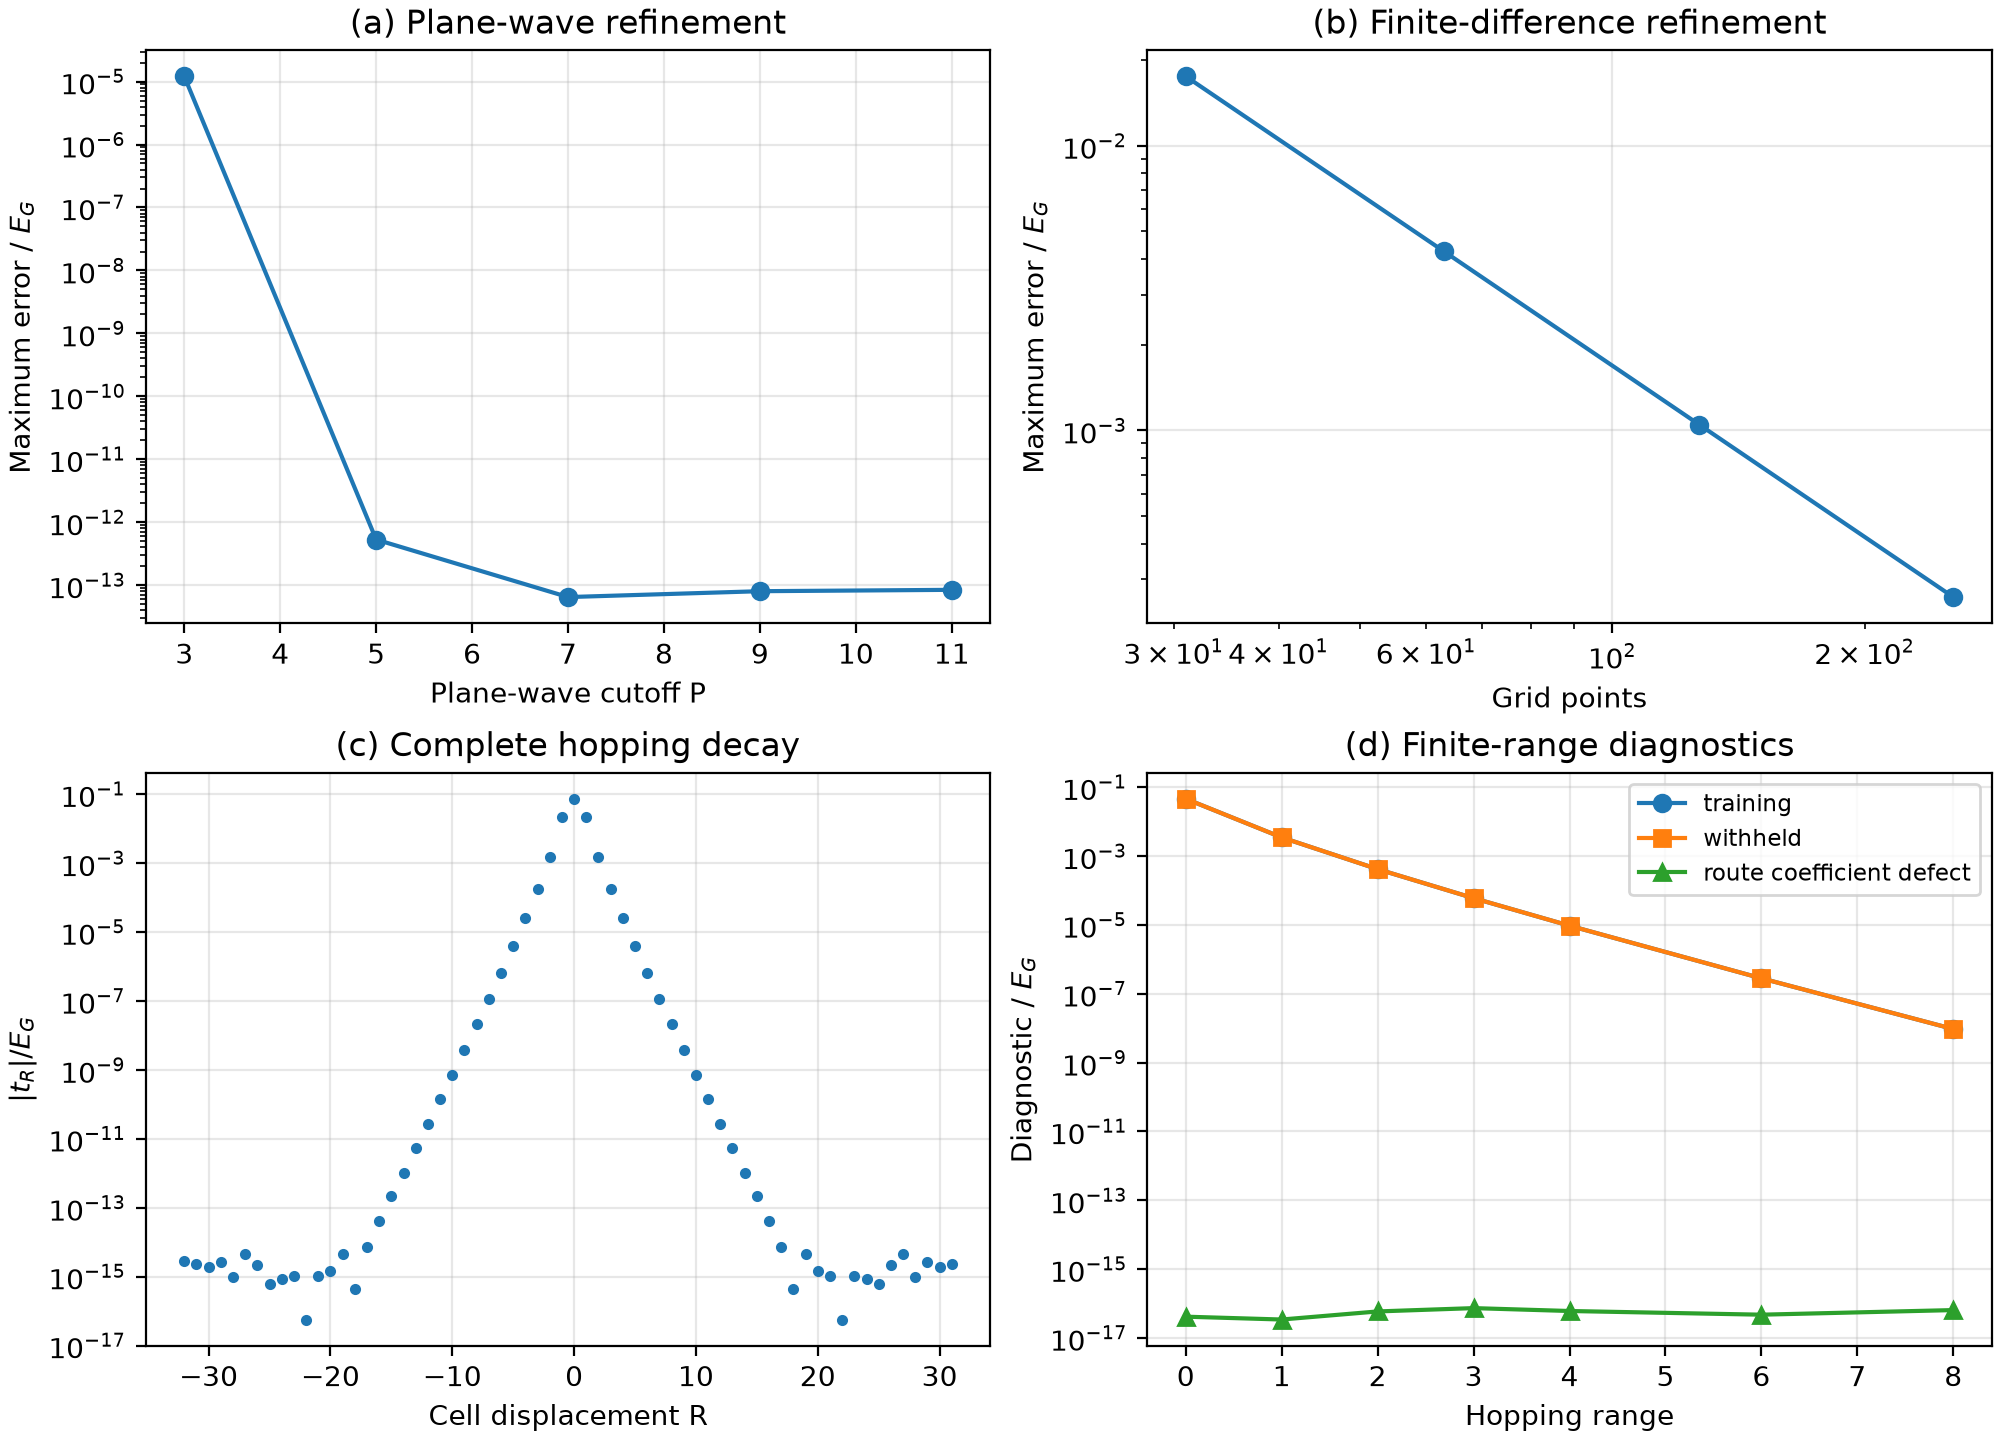
\includegraphics[width=0.97\linewidth]{../../../../../calculations/ICMSEP2026/conference/paper_1/isolated-band/isolated-band-summary.png}
 \caption{Frozen parent-representation refinement, complete hopping decay, and
 finite-range training/withheld maximum errors for the controlled
 one-dimensional model.}
 \label{fig:periodic-1d-summary}
\end{figure}

The complete 64-point transform reconstructs the represented lowest band
within $4.17\times10^{-17}E_G$. The withheld maximum absolute error decreases
from $4.62\times10^{-2}E_G$ for the onsite-only model to
$9.47\times10^{-9}E_G$ at range $8a$. The training and withheld meshes are
disjoint. No preferred range is selected because the controlled experiment has
no application-derived acceptance threshold.

\subsection{Matched reduction routes}
\label{sec:matched-routes}

Equal-weight direct least squares and Fourier-mediated truncation use the same
complete uniform mesh and Fourier model class. Under those matched conditions,
their largest coefficient defect over the frozen range sequence is
$7.38\times10^{-17}E_G$, and the largest sampled maximum defect is
$1.56\times10^{-16}E_G$. This is an algebraic control under one matched objective, not evidence that
arbitrary reduction routes commute. M1 contains no changed-weight,
restricted-training, weak-potential, gap-closure, or gauge stress attack;
Supplementary Appendix~S2 states these exclusions explicitly.

\subsection{Rank-two alignment and gauge-resolved locality}
\label{sec:multiband-alignment}

M2 uses a four-state Hermitian block polynomial whose lowest two states form a
retained group. The minimum external gap is $1.057$, and the minimum singular
value among neighboring and closure overlaps is $0.99998$. A known periodic
nonidentity rotation preserves the retained projector within
$3.24\times10^{-16}$ while producing a maximum frame defect $1.506$ and a
maximum projected-operator matrix defect $0.997$ in the attacked frame.

Pointwise Procrustes alignment recovers the known inverse attack within
$6.77\times10^{-16}$ and reduces the represented-operator defect to
$9.83\times10^{-16}$. This pointwise oracle is distinct from the constrained
family containing one global unitary for the full path. The best sampled member
of that family leaves maximum frame and operator defects of $1.131$ and $0.744$,
respectively. These values diagnose the declared constrained family; they do
not establish failure of arbitrary smooth alignment.

\begin{figure}[t]
 \centering
 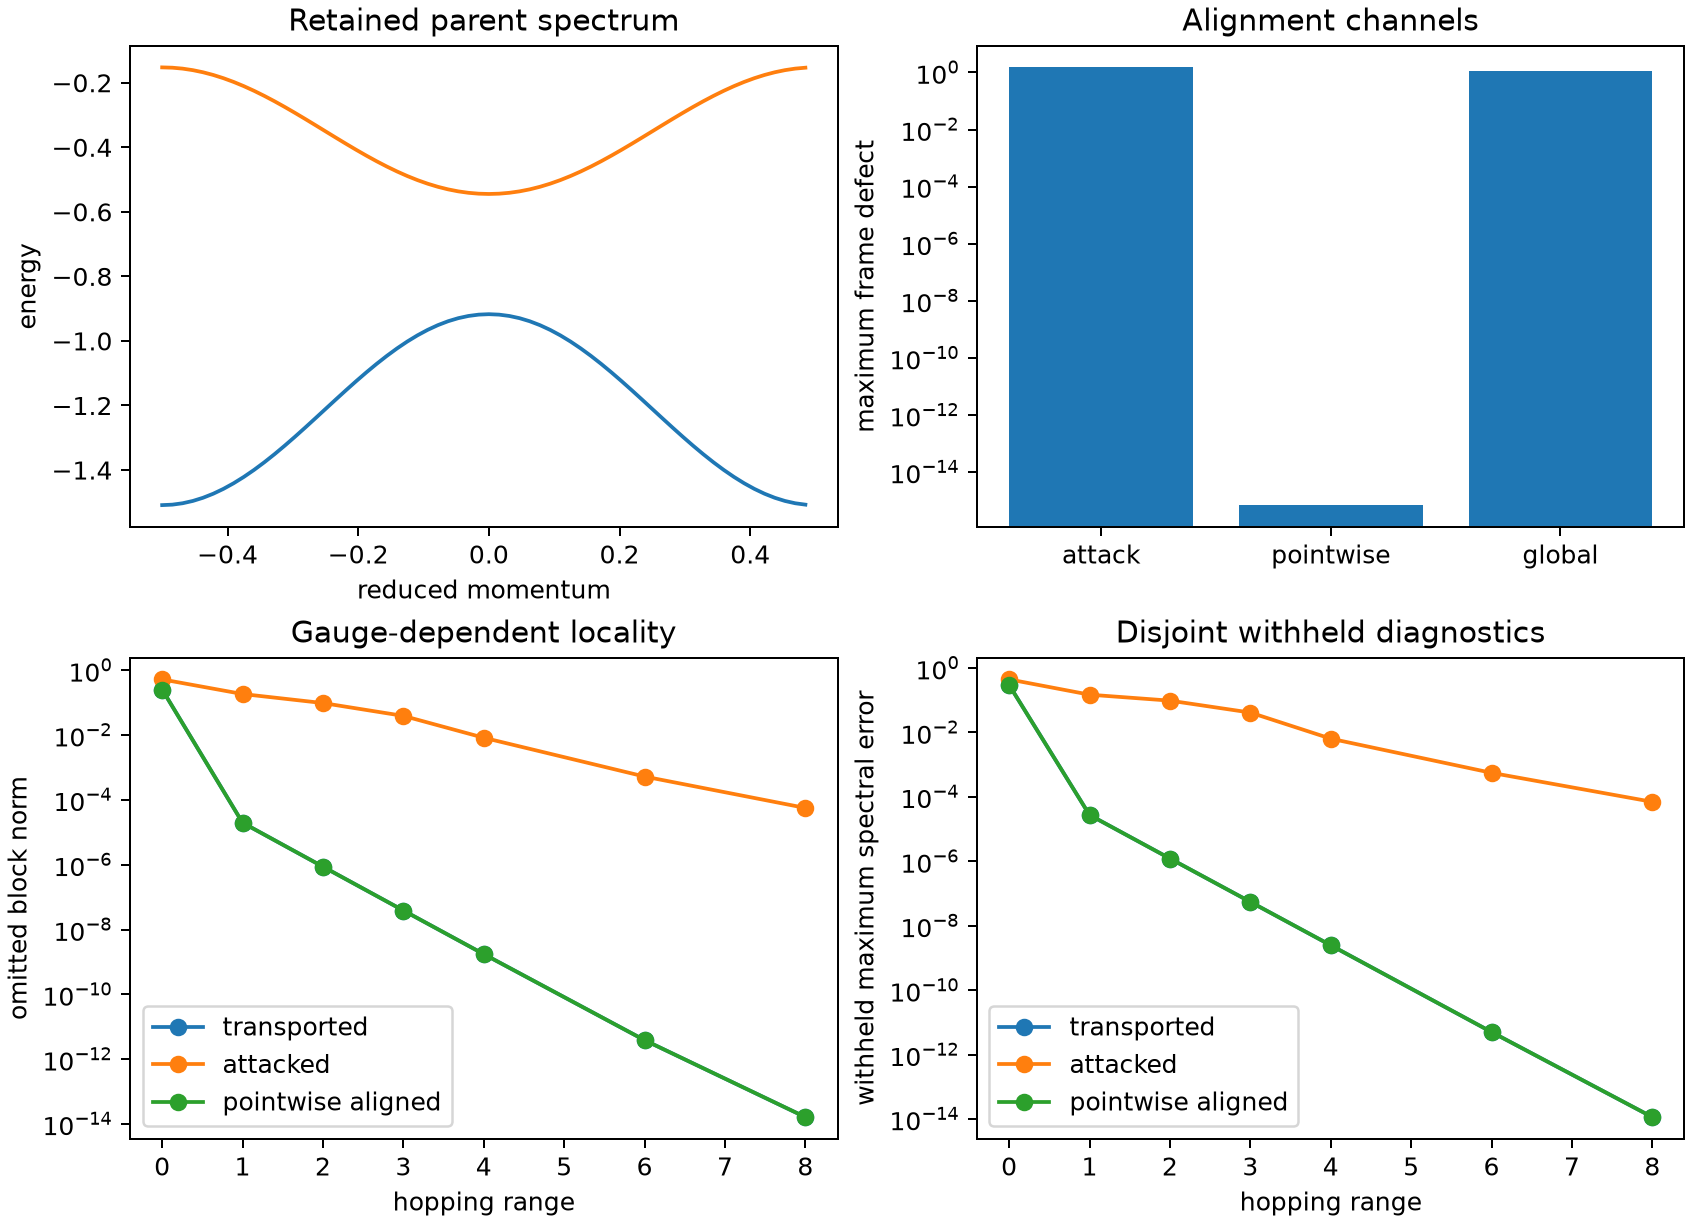
\includegraphics[width=0.97\linewidth]{../../../../../calculations/ICMSEP2026/conference/paper_1/multiband-alignment/multiband-alignment-summary.png}
 \caption{Frozen M2 retained spectrum, alignment channels, omitted block norms,
 and disjoint withheld maximum spectral errors.}
 \label{fig:multiband-alignment-summary}
\end{figure}

The known attack leaves spectra invariant but lengthens the block-hopping tail.
At range eight, its omitted-block norm and withheld maximum spectral error are
$5.65\times10^{-5}$ and $7.04\times10^{-5}$, compared with approximately
$1.6\times10^{-14}$ and $1.2\times10^{-14}$ after transport or pointwise
recovery. Independent reconstruction agrees with the retained result within
$7.43\times10^{-15}$, below the frozen $10^{-11}$ tolerance. Supplementary
Appendix~S3 gives the parent, sampling, alignment, transform, truncation,
withheld, and provenance contracts. This bounded example establishes neither a
general alignment optimizer nor material transferability.

\subsection{M3 constrained admissible sets}
\label{sec:m3-constrained-admissible-sets}

M3 composes the frozen M2 baseline with a two-parameter candidate family and
nine one-global-real-rotation components. Its thresholds are pedagogical
benchmark controls selected from the known synthetic training geometry, not
physical or uncertainty-calibrated tolerances. With spectral threshold $0.03$
and operator threshold $0.33$, the frozen point $(0,1)$ is a common witness, so the
retained compatible case has zero separation. Tightening only the operator
threshold to $0.31$ gives a \texttt{certified-separated} case with equal
analytic lower and constructive upper bounds $0.0994674$, above the
prospectively frozen resolution $0.05$. The training quadratics determine the
sets and certificate; 257 disjoint staggered evaluation coordinates remain
diagnostic only. Independent library and standalone reconstruction defects are
$1.33\times10^{-15}$ and $4.66\times10^{-15}$, below the frozen $10^{-11}$
tolerance. Supplementary Appendix~S5 records the protocol amendments, finite
certificate, locality diagnostics, and bounded evidence claim. This result is
specific to the declared synthetic family, metric, thresholds, and finite
alignment components.

\subsection{Bridge to a Wannier90-selected frame}
\label{sec:wannier90-bridge}

A separately retained synthetic two-dimensional calculation connects M2's
constructed gauge-locality mechanism to a frame selected by Wannier90 3.1.0.
It is not part of M2 and is not a first-principles calculation. The direct
projected and Wannier90 frames span the same retained subspace within a maximum
projector defect of $2.65\times10^{-10}$; pointwise alignment reduces their
represented-operator defect to $3.57\times10^{-10}E_G$. A bounded family of
integer orbital translations followed by one constant unitary instead leaves
an operator defect of $1.490E_G$, showing that this retained relation is
momentum dependent within the declared contract.

The Wannier90 frame also has the shorter retained hopping tail: at squared
radius 50 the omitted norm is $2.72\times10^{-4}E_G$, compared with
$5.90\times10^{-3}E_G$ for the direct projected frame. A six-case sensitivity
study is nonmonotone and reaches distinct localization basins, so these values
are finite-case bridge evidence rather than convergence or optimality claims.
No external program was rerun for this paper. Supplementary Appendix~S4 records
the historical authorization, portable verification, numerical channels, and
strict evidence boundary.

\subsection{Minimal analytic illustration of admissible-set decisions}
\label{sec:direct-admissible-sets}

This deliberately small benchmark illustrates the witness-versus-certificate
decision rule; it does not represent the dimensionality, gauge freedom, or
parameter complexity of the broader controlled models. It uses the scalar parent
$E_{\mathrm{ref}}(k)=1-\tfrac12\cos k+\tfrac15\cos 2k$ and the deliberately
restricted class
$E_{\bm{\theta}}(k)=\theta_0+2\theta_1\cos k$. The operator domain is
$R=-2,\ldots,2$, the canonical parameter metric is Euclidean with unit scales,
and $\mathcal{U}=\{1\}$. Exact quadratic minima are obtained before applying
the common excess-loss budget $10^{-4}$.

For equal spectral weights on the complete six-point mesh
\[
 k\in\{0,\pi/3,2\pi/3,\pi,4\pi/3,5\pi/3\},
\]
where the represented $R=0,\pm1,\pm2$ translations are distinct,
both admissible sets contain the exact witness
$(\theta_0,\theta_1)=(1,-1/4)$, so $\delta^\ast=0$. For the restricted training
set $\{-\pi/3,0,\pi/3\}$, the spectral center moves to $(3/5,1/20)$ while the
operator center remains $(1,-1/4)$. Exact rational eigenvalue enclosures and
the reverse triangle inequality certify
$0.452\leq\delta^\ast\leq0.500$. The lower bound proves separation for this
frozen contract; it is not inferred from a failed search. The restricted
spectral center has zero training residual but a withheld root-mean-square
error of $0.7211E_G$ on four disjoint points.

\begin{figure}[t]
 \centering
 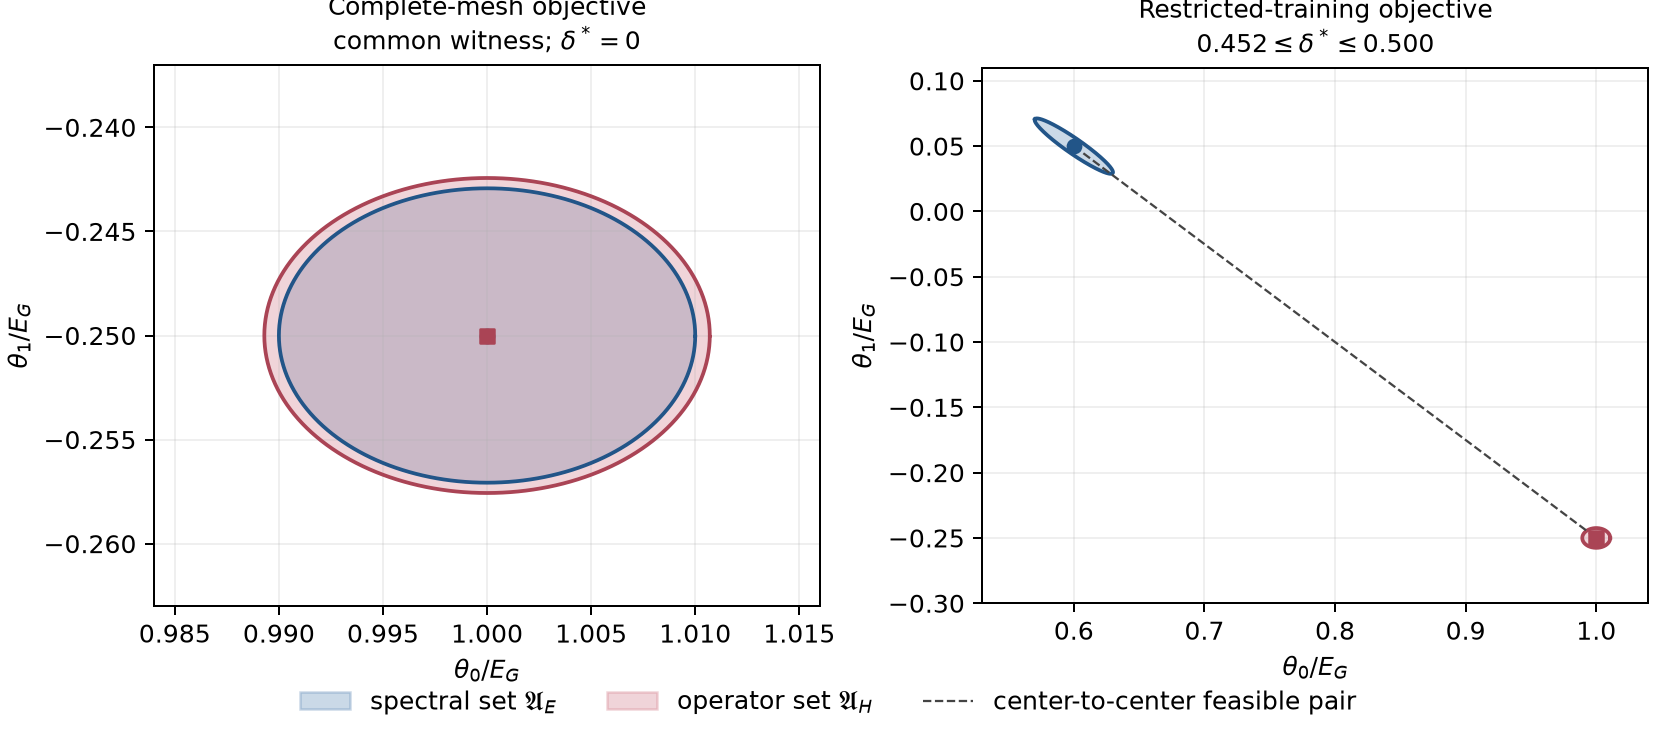
\includegraphics[width=0.97\linewidth]{../../../../../calculations/ICMSEP2026/conference/paper_1/admissible-sets.png}
 \caption{Direct analytic admissible sets. The complete-mesh case has an exact
 common witness (left); the restricted-training case has certified positive
 separation (right). Boundary samples are used only for visualization.}
 \label{fig:direct-admissible-sets}
\end{figure}

These two cases provide a minimal illustration of the asymmetric decision
logic: a common witness constructively supports compatibility, whereas a
positive lower bound is required for incompatibility. Changing only the
spectral training domain can change the disposition; neither result implies
equivalence, universal incompatibility, or broad instantiation of the framework.

\subsection{Two-dimensional coupling and shell hierarchy}
\label{sec:two-dimensional-coupling}

The two-dimensional family is
\begin{equation}
 \hat{H}_{2\mathrm{D}}
 =-\nabla^2+0.5\cos x+0.5\cos y
 +\lambda_{xy}\cos x\cos y.
 \label{eq:two-dimensional-model}
\end{equation}
At $\lambda_{xy}=0$, the represented Kronecker-sum defect is zero and the
complete product-spectrum defect is $3.55\times10^{-14}E_G$. A rank-two
degeneracy control preserves the cluster projector under a Hadamard rotation
even though the individual-vector overlap is only $1/\sqrt{2}$.

As $\lambda_{xy}$ increases from zero to 0.30, the mixed-direction hopping
norm grows from a $3.00\times10^{-15}E_G$ numerical floor to
$1.94\times10^{-3}E_G$. At the strongest coupling, the withheld
root-mean-square error decreases from $5.75\times10^{-2}E_G$ for the onsite
shell to $1.70\times10^{-6}E_G$ for the full finite transform. The full transform reconstructs its own $15\times15$ mesh within
$1.11\times10^{-15}E_G$, yet the separately evaluated $31\times31$ withheld
mesh retains the $1.70\times10^{-6}E_G$ error. This distinguishes the observed
reciprocal-mesh interpolation error from hopping truncation.

\begin{figure}[t]
 \centering
 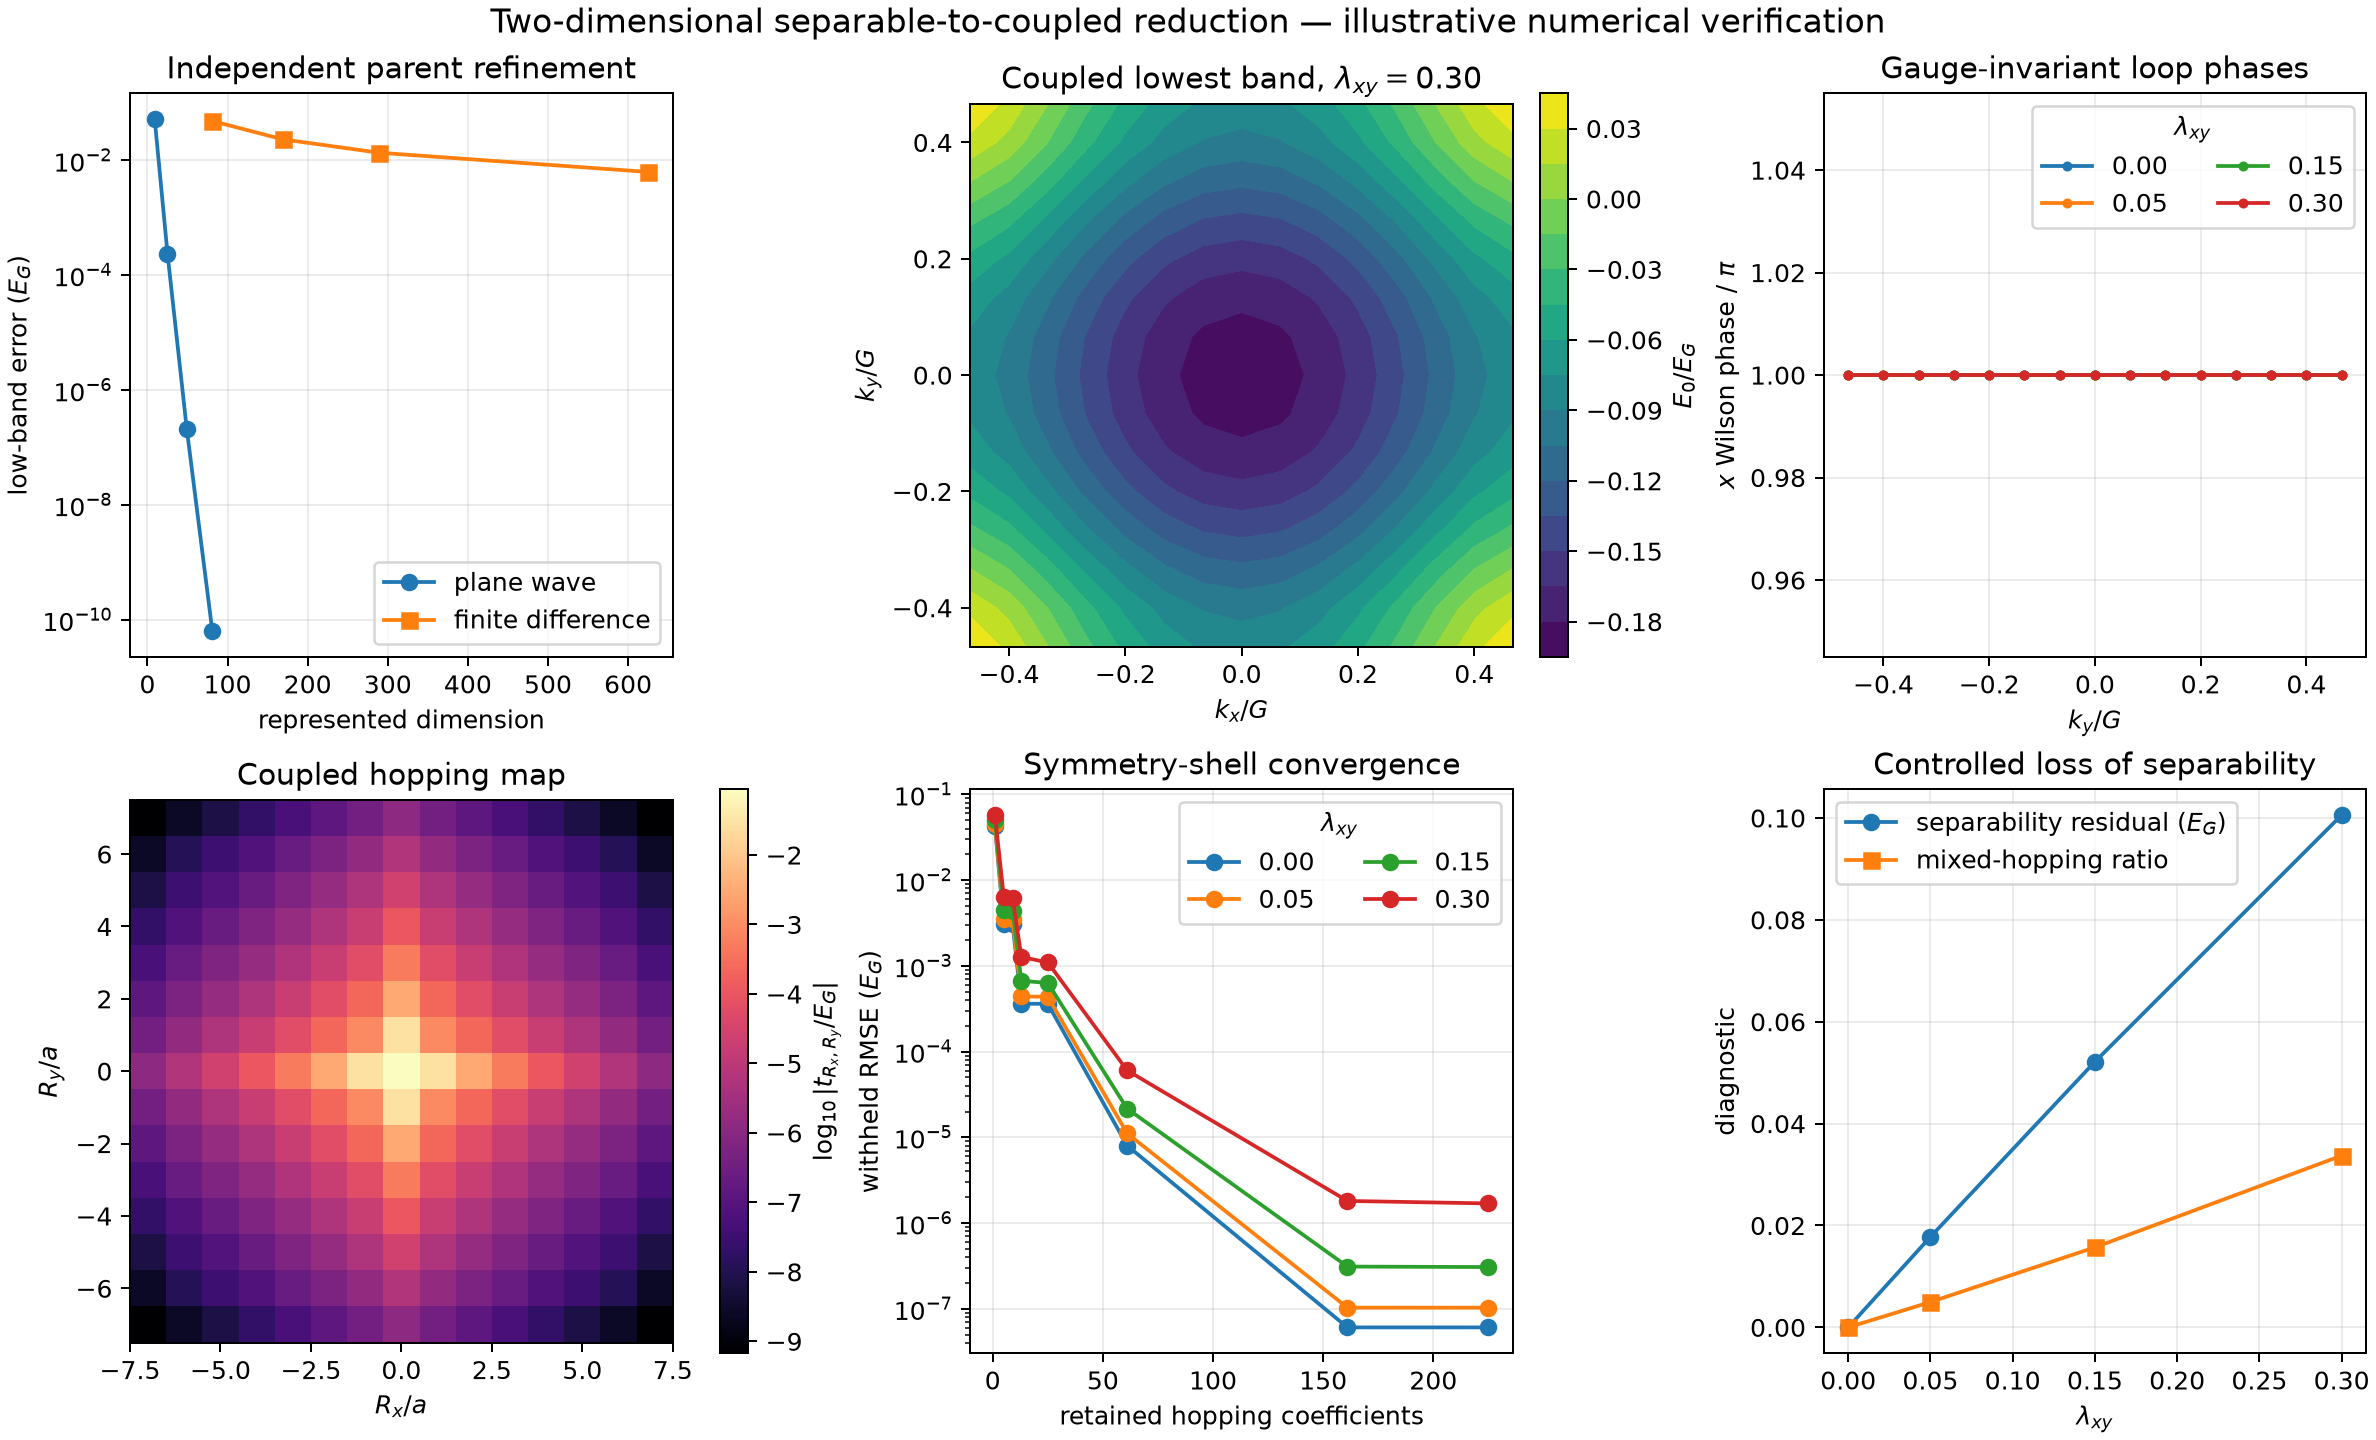
\includegraphics[width=0.97\linewidth]{../../../../../calculations/research-monograph/periodic-2d/summary.png}
 \caption{Parent refinement, coupled band surface, Wilson-loop diagnostics,
 hopping map, shell convergence, and separability controls for the synthetic
 two-dimensional family.}
 \label{fig:periodic-2d-summary}
\end{figure}

An anisotropic control gives principal masses $1.184m$ and $2.112m$ while
preserving time reversal and both reflections within
$3.60\times10^{-14}E_G$. This distinguishes tensor anisotropy from
coupling-generated mixed hopping. Together with the one-dimensional route
attacks, the shell hierarchy is central evidence that coordinate
transformation, truncation, and fitting objective must remain distinct.

\subsection{Composite gauge and locality}
\label{sec:composite-gauge}

The lowest-three-band composite test compares a smooth projected frame with a
periodic rough internal gauge. Mesh spectra agree within
$1.22\times10^{-15}E_G$, and the unordered eigenphase sets of the discrete
Wilson loops agree within $2.22\times10^{-15}$. The net eigenphase winding
gives zero total Chern diagnostic for both frames on the declared mesh. The
geometric-phase and topological interpretation follows
Refs.~\cite{resta1994,zak1989,thouless1982,niu1985}. Locality differs:
total finite-supercell spread grows from $24.90a^2$ to $67.70a^2$, while the
omitted hopping-block norm at squared-radius shell 18 grows from
$1.38\times10^{-2}E_G$ to $5.25\times10^{-1}E_G$. The spread comparison uses
the gauge-dependent localization functional introduced for composite Wannier
functions~\cite{marzari1997} and studied mathematically in
Ref.~\cite{panati2013}.

\begin{figure}[t]
 \centering
 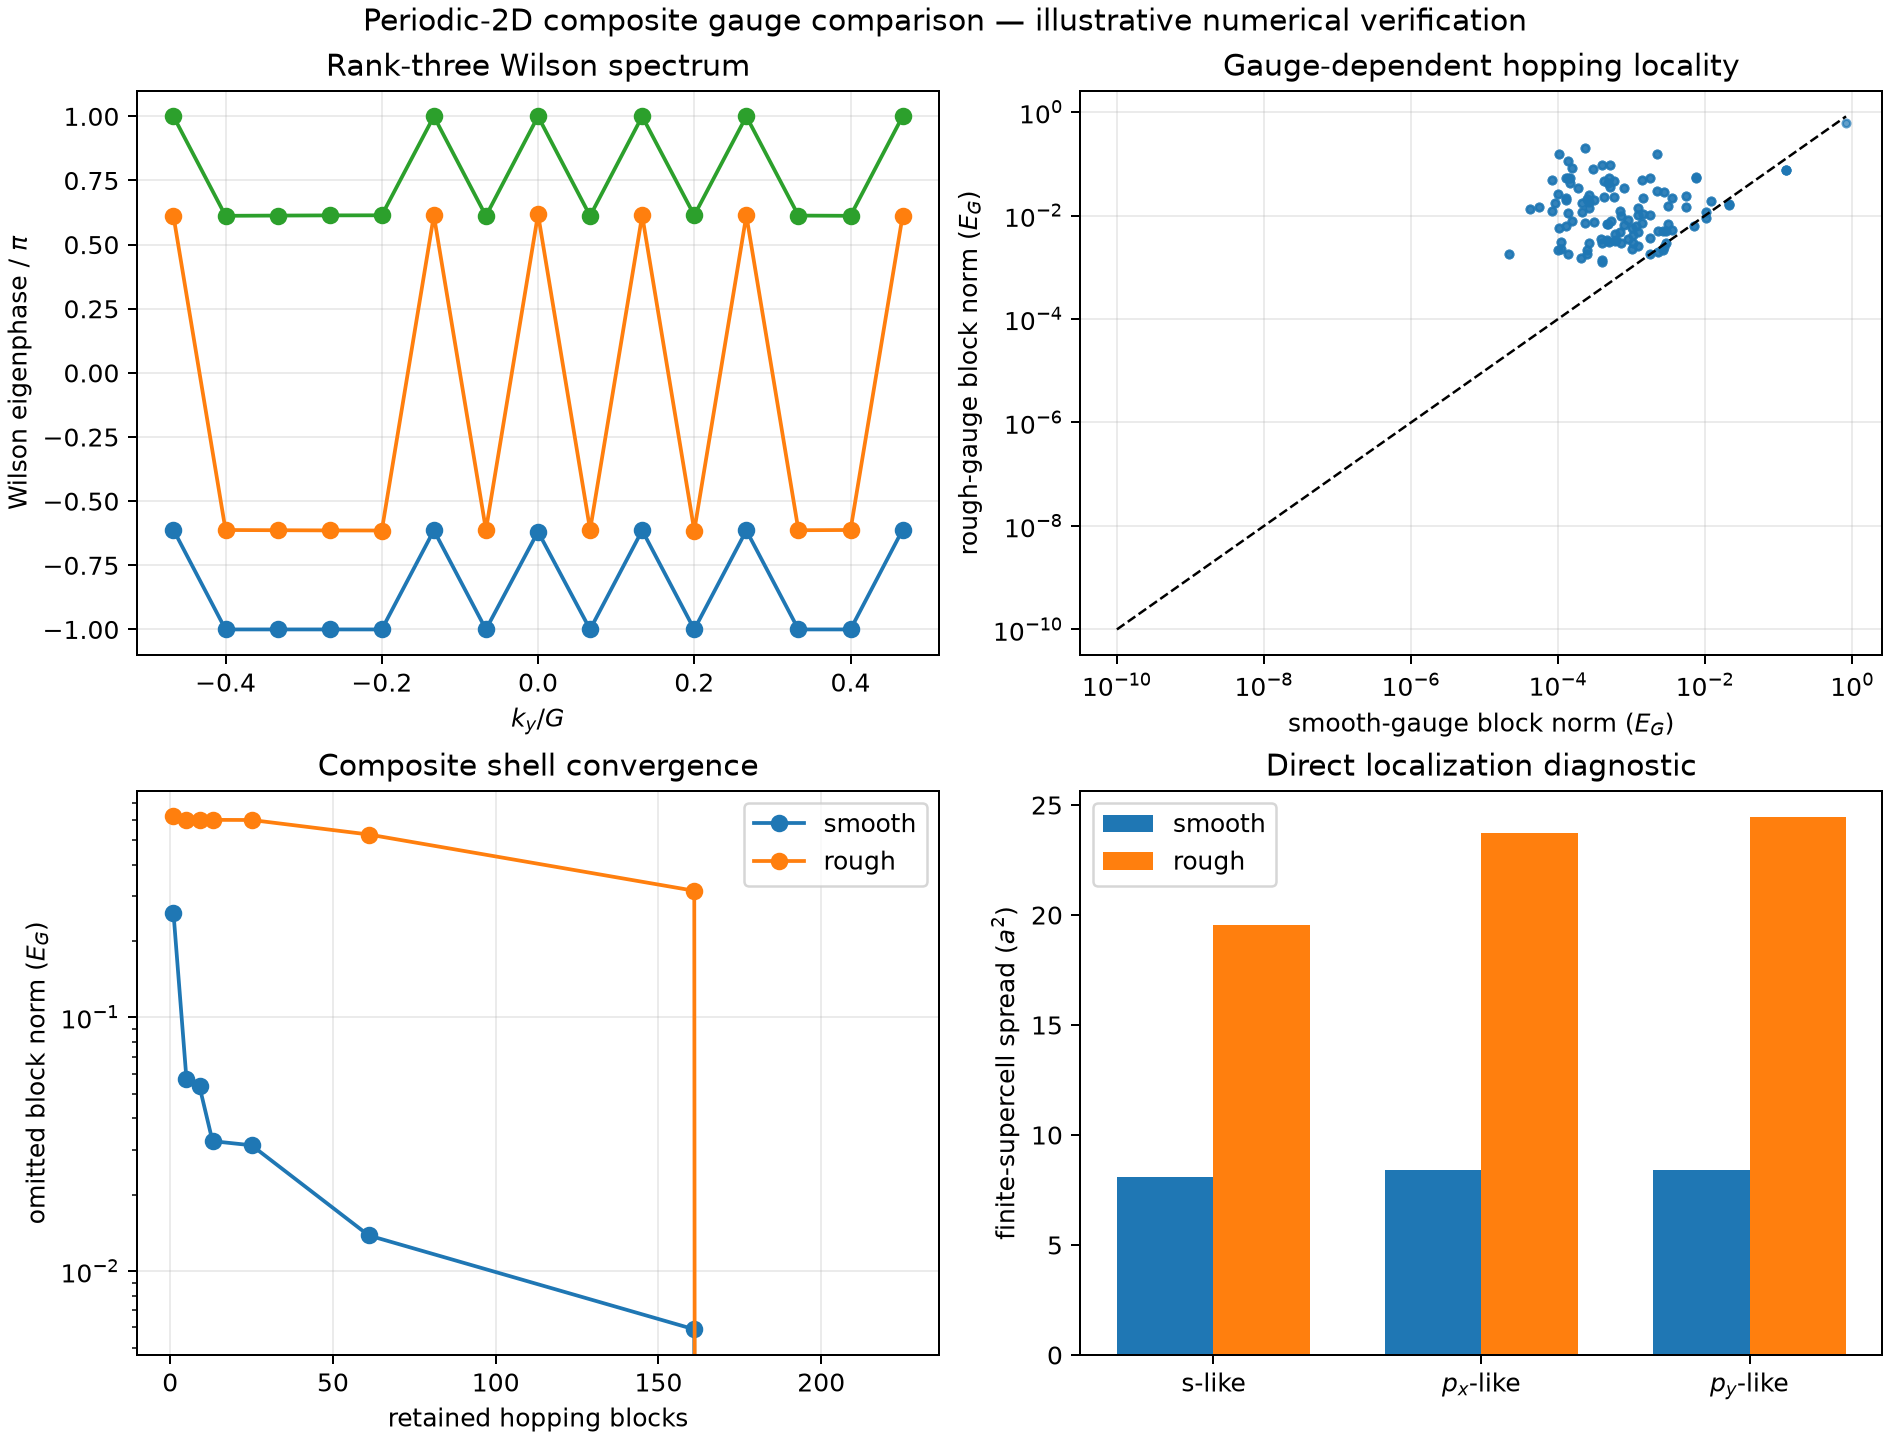
\includegraphics[width=0.97\linewidth]{../../../../../calculations/research-monograph/periodic-2d/composite-summary.png}
 \caption{Gauge-invariant subspace and spectral data coexist with strongly
 gauge-dependent localization and finite-range behavior.}
 \label{fig:periodic-2d-composite}
\end{figure}

This gauge-locality result, together with the route and truncation results, is
a principal controlled finding of the paper. Spectral equality does not
determine locality or a useful short-range representation. It also shows why
alignment freedom must be constrained before operator residuals are interpreted.

\subsection{Evidence summary}
\label{sec:evidence-summary}

\begin{table}[t]
\centering
\caption{Scope of the retained controlled-model evidence.}
\label{tab:evidence-scope}
\begin{tabular}{@{}
>{\raggedright\arraybackslash}p{0.25\textwidth}
>{\raggedright\arraybackslash}p{0.30\textwidth}
>{\raggedright\arraybackslash}p{0.30\textwidth}@{}}
\toprule
Controlled component & Demonstrated property & Unsupported conclusion \\
\midrule
Independent parent refinement
& Numerical parent errors can be separated
& Material convergence \\
Common-space alignment
& Operator residuals follow a declared identification
& Automatic physical equivalence \\
Complete and truncated hoppings
& Coordinate transformation and reduction are distinct
& Universal hopping cutoff \\
Matched construction routes
& Agreement under identical frozen objectives
& Generic commuting reductions \\
Rank-two gauge attack
& Invariant spectra can coexist with frame-dependent locality
& General alignment or material validation \\
M3 constrained admissible sets
& A finite alignment family can retain a common witness or certified separation
& Unrestricted alignment or material-level compatibility \\
Direct admissible sets
& Exact intersection and certified separation can both occur
& Contract-independent compatibility \\
\bottomrule
\end{tabular}
\end{table}

The evidence has two complementary roles. The one- and two-dimensional route,
truncation, shell, and gauge-locality studies are the primary numerical results;
they were not designed as thresholded admissible-set maps. The direct
two-parameter calculation is a minimal analytic illustration that maps two
quadratic sets, retains an exact intersection witness, and certifies a positive
lower separation bound in the changed-training case. It does not itself exercise a
nonidentity alignment or a multiband candidate. M2 supplies those controlled
alignment and locality channels but not thresholded admissible sets. M3
supplies thresholded rank-two admissible sets for a bounded two-parameter,
nine-component family, not material-relevant parameter complexity or an
unrestricted alignment search. None of these records provides a
three-dimensional material result.

\section{Conclusions and Recommendations}
\label{sec:conclusions}

Spectral and operator reductions preserve different information and should be
evaluated as separate admissible-set constraints. A valid comparison requires
common coordinates, controlled gauge freedom, explicit normalization, a finite
real-space domain, withheld checks, and bounded interpretation of optimization
evidence. A shared feasible witness supports compatibility; failure to find
one does not prove incompatibility.

The principal controlled findings are the route, truncation, shell, and
locality results. Complete representation changes can be verified independently
of finite-range approximation; direct and mediated routes agree under the
identical objectives frozen in M1 without establishing a general
commuting-reduction claim; and gauge-equivalent spectra can correspond to
substantially different localization and truncated operators.
The minimal analytic example adds a bounded demonstration that the same reduced
class can have an exact common witness under one frozen spectral objective and
certified positive separation after the training domain changes. These are
numerical-verification results for synthetic operators, not claims about a
material or a broad multiband instantiation.

M2 bridges these roles with a rank-two candidate, a known nonidentity attack,
exact pointwise recovery, and a distinct one-global-unitary constrained family.
M3 adds prospectively thresholded spectral and operator admissible sets, a
common-witness case, and a positive analytic separation certificate in a frozen
two-parameter, nine-component family. The direct map and M3 remain separate
bounded demonstrations; neither establishes that an unrestricted alignment
problem has been solved. A later first-principles silicon application must supply its own parent
convergence, Wannier validation, symmetry alignment, thresholds, and withheld
observables rather than inheriting acceptance or incompatibility from these toy
models.

\appendix
\section{Evidence and Provenance Boundary}
\label{app:evidence-provenance}

The maintained evidence is retained under:
\begin{itemize}
 \item \path{calculations/ICMSEP2026/conference/paper_1/isolated-band/};
 \item \path{calculations/ICMSEP2026/}\\
       \path{conference/paper_1/multiband-alignment/};
 \item \path{calculations/research-monograph/periodic-2d/}; and
 \item \path{calculations/ICMSEP2026/conference/paper_1/}.
\end{itemize}
Each directory contains its protocol, result records, independent verification
code, figures, report, and checksum manifest. The evidence has been classified
as controlled illustrative software and numerical verification. It is not a
public data deposit, DOI, material validation, or uncertainty analysis.

The isolated-band package contains the prospectively frozen M1 lowest-band
calculation. Its historical identity does not substitute for a retained gap or
band-isolation result. The multiband package contains the prospectively frozen
M2 rank-two alignment and
locality calculation, including its independent reconstruction and disjoint
withheld diagnostics. The two-dimensional reports contain additional composite
and topology controls.
The conference-paper parent calculation contains the direct
quadratic admissible-set map, exact common witness, rational separation
certificate, independent verifier, and figure inputs. Only the bounded results
directly used in the paper are summarized in its main text. Historical external
executions are not rerun by the manuscript.

\subsection{Verifier and digest semantics}

The standalone M1 and M2 retained verifiers decode the frozen JSON documents
and reconstruct their finite protocols without importing the corresponding
producer Actions. They remain dependent on shared numerical libraries,
runtime behavior, and declared mathematical conventions; passing establishes
bounded reconstruction consistency rather than an independent physical oracle.
The checksum manifests bind retained bytes to recorded SHA-256 digests and
therefore detect inconsistency relative to those manifests. A digest manifest
alone is not an external trusted timestamp and does not, without an independent
commit or archival record, prove when the bytes were created.

\subsection{Curation work}

The remaining evidence-curation tasks are:
\begin{itemize}
 \item[$\square$] trace every numerical statement and plotted value in the
 paper to a retained result field or report table;
 \item[$\square$] verify the figure sources against the retained checksum
 manifests;
 \item[$\square$] record the exact software revision and runtime environment
 associated with each retained calculation;
 \item[$\square$] decide which machine-readable records and figure-generation
 inputs belong in a public archival package; and
 \item[$\square$] obtain authorization before publication or deposition.
\end{itemize}
These practices follow general reproducible-computation guidance~\cite{sandve2013}.
Completing the tasks strengthens provenance and publication readiness; it does
not change the evidence class from controlled numerical verification to
material validation.

\section{Direct Admissible-Set Demonstration}
\label{app:direct-admissible-set-demonstration}

The completed controlled calculation is retained under
\path{calculations/ICMSEP2026/conference/paper_1/}. It freezes a scalar
one-dimensional parent,
\begin{equation*}
 E_{\mathrm{ref}}(k)=1-\frac12\cos k+\frac15\cos 2k,
\end{equation*}
and the two-parameter nearest-neighbor candidate family
\begin{equation*}
 E_{\bm{\theta}}(k)=\theta_0+2\theta_1\cos k.
\end{equation*}
The parameter box is
$0\leq\theta_0\leq3/2$ and $-3/4\leq\theta_1\leq1/2$. Both canonical scales
and weights are one. The operator domain is $R=-2,\ldots,2$ with unit shell
weights, and the scalar alignment family is the singleton identity.

\subsection{Frozen threshold rule}

For each quadratic loss, the exact analytic minimum is derived from the frozen
parent and sampling design. The admissibility threshold is that minimum plus
the common excess-loss budget $\epsilon=10^{-4}$. This is a controlled map
resolution, not a statistical uncertainty. The operator normalization is
global over the five translations; translation-resolved residuals and the
omitted second-neighbor tail remain separate records.

\subsection{Witness and feasible-pair certificates}

Let $\mathfrak A_E$ and $\mathfrak A_H$ denote the two frozen admissible
parameter sets and let $d$ be the declared parameter metric. If a point
$\bm\theta^\star$ satisfies both threshold inequalities, then
$\bm\theta^\star\in\mathfrak A_E\cap\mathfrak A_H$. The pair
$(\bm\theta^\star,\bm\theta^\star)$ is feasible in the definition of set
separation and has distance zero; nonnegativity of $d$ therefore proves
$\delta^\star=0$. Membership in a sampled Pareto set is neither necessary nor
sufficient for this certificate; the two threshold inequalities are the
operative hypotheses.

More generally, every feasible pair
$\bm\theta_E\in\mathfrak A_E$ and
$\bm\theta_H\in\mathfrak A_H$ gives
\begin{equation}
 \delta^\star\leq d(\bm\theta_E,\bm\theta_H).
 \label{eq:app-b-feasible-upper}
\end{equation}
Thus a sampled nondominated calculation supplies a certified upper bound only
when it supplies such a feasible pair. A distance from one sampled point to
$\mathfrak A_E\cap\mathfrak A_H$ is not a separation certificate and, when the
intersection is empty, is not the relevant quantity.

\subsection{Quadratic enclosure and separation lemma}

Suppose a frozen quadratic loss has the exact form
\begin{equation}
 \mathcal L(\bm\theta)=\mathcal L_{\min}
 +Q(\bm\theta),\qquad
 Q(\bm\theta)=(\bm\theta-\bm\theta^\star)^{\mathsf T}
 \bm G(\bm\theta-\bm\theta^\star),
 \label{eq:app-b-quadratic}
\end{equation}
where $\bm G$ is positive definite and a certified lower eigenvalue bound
$\lambda_{\min}>0$ satisfies
$Q(\bm\theta)\geq\lambda_{\min}
\|\bm\theta-\bm\theta^\star\|_2^2$. Then the threshold
$\mathcal L(\bm\theta)\leq\mathcal L_{\min}+\epsilon$ implies
\begin{equation}
 \|\bm\theta-\bm\theta^\star\|_2
 \leq r=\sqrt{\epsilon/\lambda_{\min}}.
 \label{eq:app-b-radius}
\end{equation}
Intersecting the quadratic sublevel set with the frozen parameter box can only
shrink it, so the same enclosing ball remains valid.

Apply this result to centers $\bm\theta_E^\star$ and
$\bm\theta_H^\star$ with radii $r_E$ and $r_H$. For every feasible pair, the
triangle inequality gives
\begin{align*}
 D&=\|\bm\theta_E^\star-\bm\theta_H^\star\|_2\\
 &\leq
 \|\bm\theta_E^\star-\bm\theta_E\|_2
 +\|\bm\theta_E-\bm\theta_H\|_2
 +\|\bm\theta_H-\bm\theta_H^\star\|_2\\
 &\leq r_E+\|\bm\theta_E-\bm\theta_H\|_2+r_H.
\end{align*}
Rearrangement followed by the infimum over feasible pairs proves
\begin{equation}
 \delta^\star\geq D-r_E-r_H.
 \label{eq:app-b-reverse-triangle}
\end{equation}
Consequently $D>r_E+r_H$ is a sufficient certificate of positive separation;
it does not rely on a failed search.

\subsection{Constructive compatibility case}

Equal spectral weights on the complete six-point mesh
\begin{equation*}
 k\in\{0,\pi/3,2\pi/3,\pi,4\pi/3,5\pi/3\}
\end{equation*}
keep the represented $R=0,\pm1,\pm2$ translations distinct and make the
retained first-neighbor and omitted second-neighbor Fourier columns
orthogonal. The spectral and operator sets both
contain $(\theta_0,\theta_1)=(1,-1/4)$. This exact common witness establishes
$\delta^\ast=0$ for the frozen contract. It does not establish uniqueness,
equivalence of the losses, or compatibility under another threshold or model
class.

\subsection{Certified separation case}

Changing only the spectral training domain to
$k\in\{-\pi/3,0,\pi/3\}$ moves the exact spectral center to
$(3/5,1/20)$ while leaving the operator center at $(1,-1/4)$. Their distance is
$1/2$. The restricted spectral quadratic has minimum eigenvalue
$(9-\sqrt{73})/6>91/1200$. The corresponding admissible set lies within radius
$37/1000$ of its center, while the operator set lies within radius $11/1000$ of
its center. Therefore the reverse triangle inequality certifies
\begin{equation*}
 \frac{113}{250}=0.452
 \leq\delta^\ast\leq\frac12=0.500.
\end{equation*}
The upper bound is supplied by the feasible pair of centers. The lower bound is
an exact rational enclosure, not a conclusion drawn from optimization failure
or plot resolution.

\subsection{Evidence and limitations}

The retained package contains the frozen input, protocol, result record,
independent verifier, boundary samples, figure, report, and checksum manifest.
The verifier does not import the result constructor and reconstructs the
quadratic forms, thresholds, common witness, radius inequalities, and separation
bounds. Four disjoint reciprocal points are withheld from both training sets;
they diagnose generalization and do not update either admissible set.

This demonstration is synthetic, scalar, one-dimensional, and restricted to a
singleton alignment family. It establishes both a compatible case and a
certified separated case only relative to their frozen contracts. It supplies
no three-dimensional or material-specific evidence.

\clearpage
\section*{Appendix S1. Gauge-Orbit Diagnostic Decomposition}
\label{supp:orbit-diagnostic}
\renewcommand{\theequation}{S1.\arabic{equation}}
\setcounter{equation}{0}

\subsection*{S1.1 Purpose and scope}

This appendix defines the invariant and frame-dependent parts of the operator
comparison used in the main paper. The decomposition applies to the diagnostic,
not to the Hamiltonian as a physical operator. It is defined relative to a
frozen comparison contract; changing the retained space, admissible alignment
family, weights, normalization, or finite translation domain changes the
diagnostic.

The construction is analogous in purpose to the separation of the Wannier
spread into gauge-invariant and gauge-dependent contributions
\cite{marzari1997,marzari2012,panati2013}. It is not the Wannier spread
functional and does not inherit that functional's physical or variational
interpretation.

\subsection*{S1.2 Comparison contract}

Let $V_{\mathrm{ref}}$ and $V_{\mathrm{red}}$ be retained finite-dimensional
state spaces of equal rank $r$. The operator channel requires a nonempty,
declared family
\[
 \mathcal U\subseteq
 \left\{\bm C:V_{\mathrm{red}}\rightarrow V_{\mathrm{ref}}
 \mid \bm C^\dagger\bm C=\bm C\bm C^\dagger=\bm I_r\right\}
\]
of admissible unitary identification maps. Restrictions imposed by continuity,
reciprocal-boundary sewing, symmetry, orbital semantics, or locality belong to
the definition of $\mathcal U$ rather than to a later interpretation of the
residual.

For a finite translation domain $\mathcal S_H$, nonnegative weights
$\omega_{\bm R}$, and a positive frozen normalization
\[
 Z_{\mathrm{ref}}=
 \sum_{\bm R\in\mathcal S_H}\omega_{\bm R}
 \left\|\bm H_{\mathrm{ref}}(\bm R)\right\|_{\mathrm F}^2,
\]
the aligned operator loss is
\begin{equation}
 \mathcal L_H(\bm C,\bm\theta)=
 \frac{1}{Z_{\mathrm{ref}}}
 \sum_{\bm R\in\mathcal S_H}\omega_{\bm R}
 \left\|
 \bm H_{\mathrm{ref}}(\bm R)
 -\bm C\bm H_{\mathrm{red}}(\bm R;\bm\theta)\bm C^\dagger
 \right\|_{\mathrm F}^2.
 \label{eq:supp-aligned-loss}
\end{equation}
A zero or unspecified normalization does not define this diagnostic. A
different-rank comparison likewise requires a separately declared projection
or embedding; its information loss cannot be absorbed into
Eq.~\eqref{eq:supp-aligned-loss}.

\subsection*{S1.3 Orbit loss and frame excess}

\paragraph{Attainment under a compact contract.}
For fixed $\bm\theta$, the finite-sum loss in
Eq.~\eqref{eq:supp-aligned-loss} is a continuous real-valued function of
$\bm C$. If $\mathcal U$ is nonempty and compact, the extreme-value theorem
therefore supplies $\bm C_\star\in\mathcal U$ such that
\begin{equation*}
 \inf_{\bm C\in\mathcal U}\mathcal L_H(\bm C,\bm\theta)
 =\min_{\bm C\in\mathcal U}\mathcal L_H(\bm C,\bm\theta)
 =\mathcal L_H(\bm C_\star,\bm\theta).
\end{equation*}
In the finite-rank contract used here, $U(r)$ is compact, so it is sufficient
for the admissible family to be a nonempty closed subset of $U(r)$. Sewing,
symmetry, site, and orbital restrictions imply this conclusion only when their
frozen constraint maps define a closed set; the names of those restrictions do
not by themselves prove compactness. For a merely nonempty noncompact family,
the nonnegative loss still has a well-defined infimum, but a minimizing
alignment need not exist.

For nonempty $\mathcal U$, define the contract-invariant orbit loss
\begin{equation}
 \mathcal L_{H,\mathrm{orb}}(\bm\theta)
 =\inf_{\bm C\in\mathcal U}\mathcal L_H(\bm C,\bm\theta).
 \label{eq:supp-orbit-loss}
\end{equation}
For a particular declared alignment $\bm C_0\in\mathcal U$, define the
frame-dependent excess
\begin{equation}
 \mathcal L_{H,\mathrm{frame}}(\bm C_0,\bm\theta)
 =\mathcal L_H(\bm C_0,\bm\theta)
 -\mathcal L_{H,\mathrm{orb}}(\bm\theta).
 \label{eq:supp-frame-excess}
\end{equation}
For every $\bm C_0\in\mathcal U$, the defining greatest-lower-bound
property gives
$\mathcal L_{H,\mathrm{orb}}(\bm\theta)\leq
\mathcal L_H(\bm C_0,\bm\theta)$. Subtraction therefore proves
\begin{equation}
 \mathcal L_H(\bm C_0,\bm\theta)
 =\mathcal L_{H,\mathrm{orb}}(\bm\theta)
 +\mathcal L_{H,\mathrm{frame}}(\bm C_0,\bm\theta),
 \qquad
 \mathcal L_{H,\mathrm{frame}}\geq 0.
 \label{eq:supp-loss-decomposition}
\end{equation}
This is an exact scalar decomposition of the diagnostic. It is not an
orthogonal decomposition of the residual matrix.

The orbit term is the greatest lower bound of the operator discrepancy over the
frozen admissible family. The frame term measures the excess associated with
the selected admissible representative. Both statements are relative to
$\mathcal U$: enlarging the family can decrease the orbit loss, while adding
physical restrictions can increase it.

\subsection*{S1.4 Frame invariance}

Consider independent frame changes $\bm A$ on $V_{\mathrm{ref}}$ and $\bm B$
on $V_{\mathrm{red}}$. They transform the represented operators and alignment
map as
\[
 \bm H_{\mathrm{ref}}' =\bm A\bm H_{\mathrm{ref}}\bm A^\dagger,
 \qquad
 \bm H_{\mathrm{red}}' =\bm B\bm H_{\mathrm{red}}\bm B^\dagger,
 \qquad
 \bm C'=\bm A\bm C\bm B^\dagger.
\]
If the admissible family is transported bijectively to
$\mathcal U'=\{\bm A\bm C\bm B^\dagger:\bm C\in\mathcal U\}$, then the
residual corresponding to $\bm C'=\bm A\bm C\bm B^\dagger$ is $\bm A$ times
the original residual times $\bm A^\dagger$. Unitary invariance of the
Frobenius norm gives
\[
 \mathcal L_H'(\bm C',\bm\theta)=\mathcal L_H(\bm C,\bm\theta).
\]
Because $\bm C\mapsto\bm A\bm C\bm B^\dagger$ is a bijection,
\begin{align*}
 \inf_{\bm C'\in\mathcal U'}\mathcal L_H'(\bm C',\bm\theta)
 &=\inf_{\bm C\in\mathcal U}
   \mathcal L_H'(\bm A\bm C\bm B^\dagger,\bm\theta)\\
 &=\inf_{\bm C\in\mathcal U}\mathcal L_H(\bm C,\bm\theta).
\end{align*}
Thus $\mathcal L_{H,\mathrm{orb}}$ is unchanged. Applying the same identity to
the corresponding representative
$\bm C_0'=\bm A\bm C_0\bm B^\dagger$ and subtracting the equal orbit losses
also proves equality of the two frame excesses. The numerical matrices
representing $\bm C_0$ and the residual may nevertheless change.

This invariance is contractual rather than absolute. A transformation that
violates a frozen symmetry, site, orbital, or sewing condition does not belong
to the same admissible comparison problem.

\subsection*{S1.5 Outcomes when subtraction is unavailable}

The diagnostic has three distinct outcomes:
\begin{enumerate}
 \item If $\mathcal U$ is nonempty, the orbit loss is defined. A feasible
 alignment supplies an upper bound; a certified lower bound requires a separate
 global argument.
 \item If the retained ranks differ but a scientifically authorized projection
 or embedding is supplied, comparison may proceed in the declared target space.
 Projection or embedding error remains a separate diagnostic.
 \item If no admissible identification exists, the matrix-difference channel is
 undefined. The recorded outcome is a state-space mismatch, not a large
 operator residual.
\end{enumerate}

Gauge-invariant channels can remain available in the third case. Spectra and
trace invariants may be compared after their own indexing and normalization
contracts are fixed. Projector distances require both retained subspaces to be
embedded in the same parent Hilbert space. Wilson-loop eigenphase multisets can
be compared without choosing an internal frame, provided the loop, rank, gap,
and reciprocal sewing contracts agree. These invariant channels do not create
an operator identification map by themselves.

\subsection*{S1.6 Relation to the Wannier decomposition}

For a retained Bloch subspace, the Wannier spread admits the established
separation
\[
 \Omega=\Omega_{\mathrm I}+\widetilde\Omega,
\]
where $\Omega_{\mathrm I}$ depends only on the subspace projectors and
$\widetilde\Omega$ depends on the selected Bloch frame
\cite{marzari1997,marzari2012}. Equations~\eqref{eq:supp-orbit-loss}--
\eqref{eq:supp-loss-decomposition} use the same conceptual distinction between
an equivalence class and its representative, but they answer a different
question. They quantify cross-model operator discrepancy over a declared
admissible orbit; they do not quantify Wannier localization.

Accordingly, a small orbit loss establishes agreement only for the finite
operator diagnostic that was defined. A small frame excess places the achieved
loss near the orbit infimum; it does not imply that the alignment matrix is
close to a unique optimizer. Neither quantity, by itself, establishes material
validity, continuum convergence, or locality outside the frozen comparison
domain.

\clearpage
\section*{Appendix S2. M1 Isolated-Band Calculation}
\label{supp:m1-isolated-band}
\renewcommand{\theequation}{S2.\arabic{equation}}
\setcounter{equation}{0}
\renewcommand{\thetable}{S2.\arabic{table}}
\setcounter{table}{0}

\subsection*{S2.1 Role and frozen scope}

M1 is the planning identifier for the prospectively frozen, controlled
one-dimensional lowest-band calculation used in the main paper. Its retained
calculation identity is
\begin{center}
\path{icmsep2026.paper1.periodic1d.isolated-band.v1}.
\end{center}
The calculation is synthetic numerical-verification evidence. It evaluates a
finite parent representation, extracts the lowest scalar band, performs a
complete reciprocal-to-hopping transform, constructs finite-range reductions,
compares matched routes, and evaluates disjoint withheld points. The retained
schema contains no band-gap result and does not by itself establish that this
lowest band is isolated; a sampled-gap or stronger isolation argument is a
separate prerequisite channel. The historical identity is not reinterpreted as
such evidence. The calculation contains no material parameters or external
electronic-structure execution.

The dimensionless parent is
\begin{equation}
 \widehat H(k)=-\frac{\mathrm d^2}{\mathrm d x^2}+0.5\cos x,
 \qquad a=2\pi,\quad G=1,\quad E_G=1.
 \label{eq:supp-m1-parent}
\end{equation}
Reduced momentum $k/G$ lies in $[-1/2,1/2]$. The energy zero is fixed by the
model; no post-calculation energy shift is fitted. Table~\ref{tab:supp-m1-controls}
collects the controls frozen before confirmatory execution.

\begin{table}[ht]
\centering
\caption{Prospectively frozen M1 controls.}
\label{tab:supp-m1-controls}
\begin{tabular}{@{}ll@{}}
\toprule
Control & Frozen value \\
\midrule
Plane-wave cutoffs & $3,5,7,9,11$ \\
Finite represented reference cutoff & $15$ \\
Production plane-wave cutoff & $11$ \\
Finite-difference grids & $31,63,127,255$ points \\
Parent momenta & $-1/2,-1/4,0,1/4,1/2$ \\
Compared parent bands & lowest three ordered bands \\
Training mesh & 64-point centered half-open mesh \\
Hopping ranges & $0,1,2,3,4,6,8$ \\
Withheld mesh & 257-point staggered uniform mesh \\
Numerical-consistency tolerance & $10^{-12}$ \\
Coordinate tolerance & $10^{-14}$ \\
\bottomrule
\end{tabular}
\end{table}

The historical Mathieu values, common-low-mode comparison, weak-potential
sweep, and stress attacks are outside M1. Multiband alignment, nonidentity gauge
families, Wannier localization, topology, two-dimensional shells, material
validation, and uncertainty quantification are also outside its frozen scope.

\subsection*{S2.2 Parent-representation diagnostics}

At each frozen momentum, the lowest three eigenvalues were compared with the
cutoff-15 plane-wave representation. This cutoff is the declared finite
reference for M1, not an exact continuum spectrum. The plane-wave observations
are listed in Table~\ref{tab:supp-m1-plane-wave}.

\begin{table}[ht]
\centering
\caption{Maximum absolute plane-wave spectral discrepancy relative to the
cutoff-15 represented reference.}
\label{tab:supp-m1-plane-wave}
\begin{tabular}{@{}rr@{}}
\toprule
Cutoff $P$ & Maximum discrepancy ($E_G$) \\
\midrule
3  & $1.2107868154753731\times10^{-5}$ \\
5  & $5.311306949806749\times10^{-13}$ \\
7  & $6.483702463810914\times10^{-14}$ \\
9  & $8.038014698286133\times10^{-14}$ \\
11 & $8.448797217397441\times10^{-14}$ \\
\bottomrule
\end{tabular}
\end{table}

The cutoff-7 through cutoff-11 discrepancies fluctuate at the represented
binary64 scale, so this sequence is not interpreted as a monotone continuum
error estimate. The independently assembled centered finite-difference channel
produced Table~\ref{tab:supp-m1-fd}.

\begin{table}[ht]
\centering
\caption{Maximum absolute finite-difference spectral discrepancy relative to
the same cutoff-15 represented reference.}
\label{tab:supp-m1-fd}
\begin{tabular}{@{}rr@{}}
\toprule
Grid points & Maximum discrepancy ($E_G$) \\
\midrule
31  & $1.75327419749558\times10^{-2}$ \\
63  & $4.2534045602447\times10^{-3}$ \\
127 & $1.0471636947908536\times10^{-3}$ \\
255 & $2.597716946719508\times10^{-4}$ \\
\bottomrule
\end{tabular}
\end{table}

The observed decrease is the finite-grid refinement diagnostic. M1 does not
convert it into a continuum convergence certificate.

\subsection*{S2.3 Training and withheld roles}

The 64-point training mesh supplies the complete discrete Fourier transform and
the equal-weight direct fits. For training extent $N=64$ and withheld extent
$M=257$, withheld coordinate $i$ is
\begin{equation}
 \frac{k_i}{G}=-\frac12+\frac{i+1/(N+1)}{M},
 \qquad i=0,\ldots,M-1.
 \label{eq:supp-m1-withheld}
\end{equation}
The retained verifier confirms that the training and withheld coordinates are
disjoint. Withheld values enter evaluation only; they do not alter coefficients,
ranges, tolerances, or figure selection.

The complete scalar hopping coefficients are
\begin{equation}
 t_R=\frac{1}{N}\sum_{j=0}^{N-1}
 e^{-2\pi iRk_j/G}E(k_j).
 \label{eq:supp-m1-transform}
\end{equation}
For the centered half-open mesh $k_j/G=-1/2+j/N$, the Fourier columns obey
\begin{equation}
 \frac{1}{N}\sum_{j=0}^{N-1}
 e^{2\pi i(S-R)k_j/G}
 =(-1)^{S-R}\,\delta_{R,S\ (\mathrm{mod}\ N)}.
 \label{eq:supp-m1-fourier-orthogonality}
\end{equation}
Thus distinct retained representatives modulo $N$ are orthogonal; the centered
origin contributes the factor $(-1)^{S-R}$. Their inverse transform reconstructs
the training samples with maximum absolute error
$4.166137705498387\times10^{-17}E_G$. The maximum modular Hermiticity defect is
$2.0907097393389345\times10^{-18}E_G$.

For each range $R_{\max}$, the mediated route truncates the complete
coefficients to $|R|\leq R_{\max}$. The direct route fits those same
representatives by equal-weight complex least squares on the same training
mesh. Tables~\ref{tab:supp-m1-ranges} and
\ref{tab:supp-m1-route-defects} report the retained range diagnostics.

\begin{table}[ht]
\centering
\small
\caption{M1 finite-range error and omitted-block diagnostics. All diagnostic
columns have energy unit $E_G$.}
\label{tab:supp-m1-ranges}
\begin{tabular}{@{}rrrr@{}}
\toprule
$R_{\max}$ & Training maximum & Withheld maximum & Omitted-block norm \\
\midrule
0 & $4.6235761235\times10^{-2}$ & $4.6235757038\times10^{-2}$ & $3.0304371874\times10^{-2}$ \\
1 & $3.4907261092\times10^{-3}$ & $3.4907249362\times10^{-3}$ & $2.1876792983\times10^{-3}$ \\
2 & $4.1809353421\times10^{-4}$ & $4.1809323067\times10^{-4}$ & $2.5574448521\times10^{-4}$ \\
3 & $6.0054872741\times10^{-5}$ & $6.0054797140\times10^{-5}$ & $3.6185634797\times10^{-5}$ \\
4 & $9.5136496848\times10^{-6}$ & $9.5136312847\times10^{-6}$ & $5.6738480443\times10^{-6}$ \\
6 & $2.8158443985\times10^{-7}$ & $2.8158339337\times10^{-7}$ & $1.6575039069\times10^{-7}$ \\
8 & $9.4653549651\times10^{-9}$ & $9.4652957590\times10^{-9}$ & $5.5272060152\times10^{-9}$ \\
\bottomrule
\end{tabular}
\end{table}

\begin{table}[ht]
\centering
\caption{M1 direct-versus-mediated coefficient defects.}
\label{tab:supp-m1-route-defects}
\begin{tabular}{@{}rr@{}}
\toprule
$R_{\max}$ & Coefficient defect ($E_G$) \\
\midrule
0 & $4.1633363423\times10^{-17}$ \\
1 & $3.4428416195\times10^{-17}$ \\
2 & $5.9106172771\times10^{-17}$ \\
3 & $7.3812041610\times10^{-17}$ \\
4 & $6.0865104451\times10^{-17}$ \\
6 & $4.7557874187\times10^{-17}$ \\
8 & $6.4715834978\times10^{-17}$ \\
\bottomrule
\end{tabular}
\end{table}

Across the frozen sequence, the largest direct-versus-mediated coefficient
defect is $7.38120416098117\times10^{-17}E_G$, and the largest sampled maximum
route defect is $1.564917933602745\times10^{-16}E_G$. The largest Parseval
residual is $6.938893903907228\times10^{-18}E_G^2$, and the largest imaginary
band-shape residual is $9.479926314907974\times10^{-16}E_G$. These are matched-
route and numerical-consistency diagnostics. M1 defines no preferred hopping
range or scientific acceptance threshold.

\subsection*{S2.4 Independent reconstruction and provenance}

The retained verifier strictly decodes the frozen input and result documents
and imports neither the producer entry point nor the maintained
\texttt{ksdft2effmass} calculation implementation. It independently rebuilds
parent matrices, spectra, Fourier coefficients, truncations, least-squares
fits, route defects, Hermiticity, Parseval quantities, and band-shape
diagnostics. It nevertheless shares NumPy, SciPy, eigensolver semantics,
model conventions, and the runtime environment with the producer; it is an
independent finite-protocol reconstruction, not an independent physical or
continuum oracle. The verification passed with the defects in
Table~\ref{tab:supp-m1-verification}.

\begin{table}[ht]
\centering
\caption{Independent retained-reconstruction defects.}
\label{tab:supp-m1-verification}
\begin{tabular}{@{}lr@{}}
\toprule
Reconstructed channel & Maximum absolute defect \\
\midrule
Spectral & $0$ \\
Hopping & $4.781392881215698\times10^{-17}$ \\
Diagnostic & $2.731148640577885\times10^{-14}$ \\
\bottomrule
\end{tabular}
\end{table}

All are below the frozen $10^{-12}$ verification tolerance. The result and
verification wire identities are
\begin{center}
\path{ksdft2effmass.periodic1d.isolated-band-calculation-result.v1},\\
\path{ksdft2effmass.periodic1d.isolated-band-calculation-verification.v1}.
\end{center}
The protocol-freeze record contains the hashes of \path{input.json} and
\path{protocol.md} recorded before confirmatory execution. The retained package
further binds the result, verification, scripts, software record, source
manifest, figure data, and figure through \path{SHA256SUMS}. These digests test
byte identity relative to the retained manifests; by themselves they do not
supply an external trusted timestamp or prove chronology. The source manifest
records the calculation snapshot and is not a claim that a later evolving
worktree has identical hashes. The calculation used local in-process Python
software only; it invoked no external electronic-structure calculator,
scheduler, remote resource, or material dataset.

\clearpage
\section{M2 multiband alignment and gauge-resolved locality}
\label{app:supp-m2}

\subsection{Identity and evidence boundary}

M2 is the prospectively frozen local synthetic calculation with identity
\begin{center}
 \small\path{icmsep2026.paper1.periodic1d.}\\
 \path{multiband-alignment.v1}
\end{center}
Its retained package is
\begin{center}
 \small\path{calculations/ICMSEP2026/conference/paper_1/}\\
 \path{multiband-alignment/}.
\end{center}
The producer composes maintained frame transport, pointwise alignment,
operator projection, Fourier transformation, block-hopping truncation,
interpolation, and band-error Actions. The retained verifier reconstructs the
finite protocol without calling the producer Action.

M2 establishes bounded numerical behavior for one constructed rank-two
example. It does not establish material validity, uncertainty bounds,
continuum convergence, a general nonconvex alignment solver, or scientific
acceptance. In particular, the exact pointwise Procrustes channel is kept
separate from the constrained family containing one global unitary over the
whole reciprocal path.

\subsection{Gapped parent and frozen sampling}

The four-state parent is the block polynomial
\begin{equation}
 H(k)=T_0+e^{2\pi i k}T_1+e^{-2\pi i k}T_1^\dagger,
 \qquad k\in[-1/2,1/2),
 \label{eq:supp-m2-parent}
\end{equation}
with
\begin{equation}
 T_0=\begin{pmatrix}
 -1.20&0.06&0&0\\0.06&-0.35&0&0\\
 0&0&1.00&0.04\\0&0&0.04&1.75
 \end{pmatrix},\quad
 T_1=\begin{pmatrix}
 0.15&0&0&0\\0&-0.10&0&0\\
 0.12&0&0.05&0\\0&0.10&0&-0.04
 \end{pmatrix}.
 \label{eq:supp-m2-blocks}
\end{equation}
The two lowest eigenstates define the retained composite space. The training
mesh has 64 centered half-open points. The 257 withheld points use the frozen
staggered rule recorded in the result and are disjoint from training. The
observed minimum separation between the retained group and the upper group is
$1.0566461211497047$, above the frozen lower bound $0.5$. The minimum singular
value among neighboring and closure overlaps is
$0.9999828868735376$, above the frozen transport threshold $0.8$.

\subsection{Sewing, transport, and known gauge attack}

Raw retained eigenframes are polar transported along the ordered mesh and
closed using identity reciprocal-boundary sewing. For transported frame
$U(k)$, the known periodic attack is
\begin{equation}
 \widetilde U(k)=U(k)A(k),\qquad
 A(k)=\begin{pmatrix}\cos\theta(k)&-\sin\theta(k)\\
 \sin\theta(k)&\cos\theta(k)\end{pmatrix},
 \label{eq:supp-m2-attack}
\end{equation}
where
\begin{equation}
 \theta(k)=0.30+0.65\sin(2\pi k)+0.30\sin(4\pi k).
 \label{eq:supp-m2-angle}
\end{equation}
The projector defect between $U$ and $\widetilde U$ is
$3.24\times10^{-16}$, while their maximum frame defect is $1.506$.
Thus the retained state space is unchanged although its matrix frame changes.
The closure eigenphases are $0.01416$ and $0.01878$ radians; they are retained
as finite-mesh transport diagnostics, not as a topological classification.

At each point, Procrustes alignment recovers $A(k)^\dagger$ with maximum
rotation defect $6.77\times10^{-16}$. The aligned-frame defect is
$7.00\times10^{-16}$. By contrast, the separately frozen constrained family
uses one global unitary $C$ for all points. Its optimum for the sampled path is
numerically the constant rotation by $-0.30$ radians, and its maximum frame
defect remains $1.131$. This comparison diagnoses the limitation of that
specific constrained family; it is not a failed global search over arbitrary
smooth gauges.

\subsection{Projected operators and complete block hoppings}

For each frame $V(k)$, the represented retained operator is
\begin{equation}
 H_V(k)=V(k)^\dagger H(k)V(k).
 \label{eq:supp-m2-projected}
\end{equation}
The attacked representation differs from the transported representation by a
maximum Frobenius defect $0.9972$, although their unordered spectra are
identical. Pointwise alignment reduces this matrix defect to
$9.83\times10^{-16}$. The one-global-unitary channel leaves a maximum defect
$0.7443$. These are frame-dependent matrix diagnostics after explicit
identification; the common projector and spectra are invariant channels.

Complete 64-point Fourier transforms reconstruct the transported, attacked,
and pointwise-aligned matrix samples with maximum Frobenius errors
$6.76\times10^{-16}$, $1.14\times10^{-15}$, and
$6.77\times10^{-16}$, respectively. Their block-Hermiticity defects are at
most $4.50\times10^{-17}$. Complete reconstruction verifies the finite
discrete transform; it does not establish unsampled continuum interpolation.

\begin{figure}[t]
 \centering
 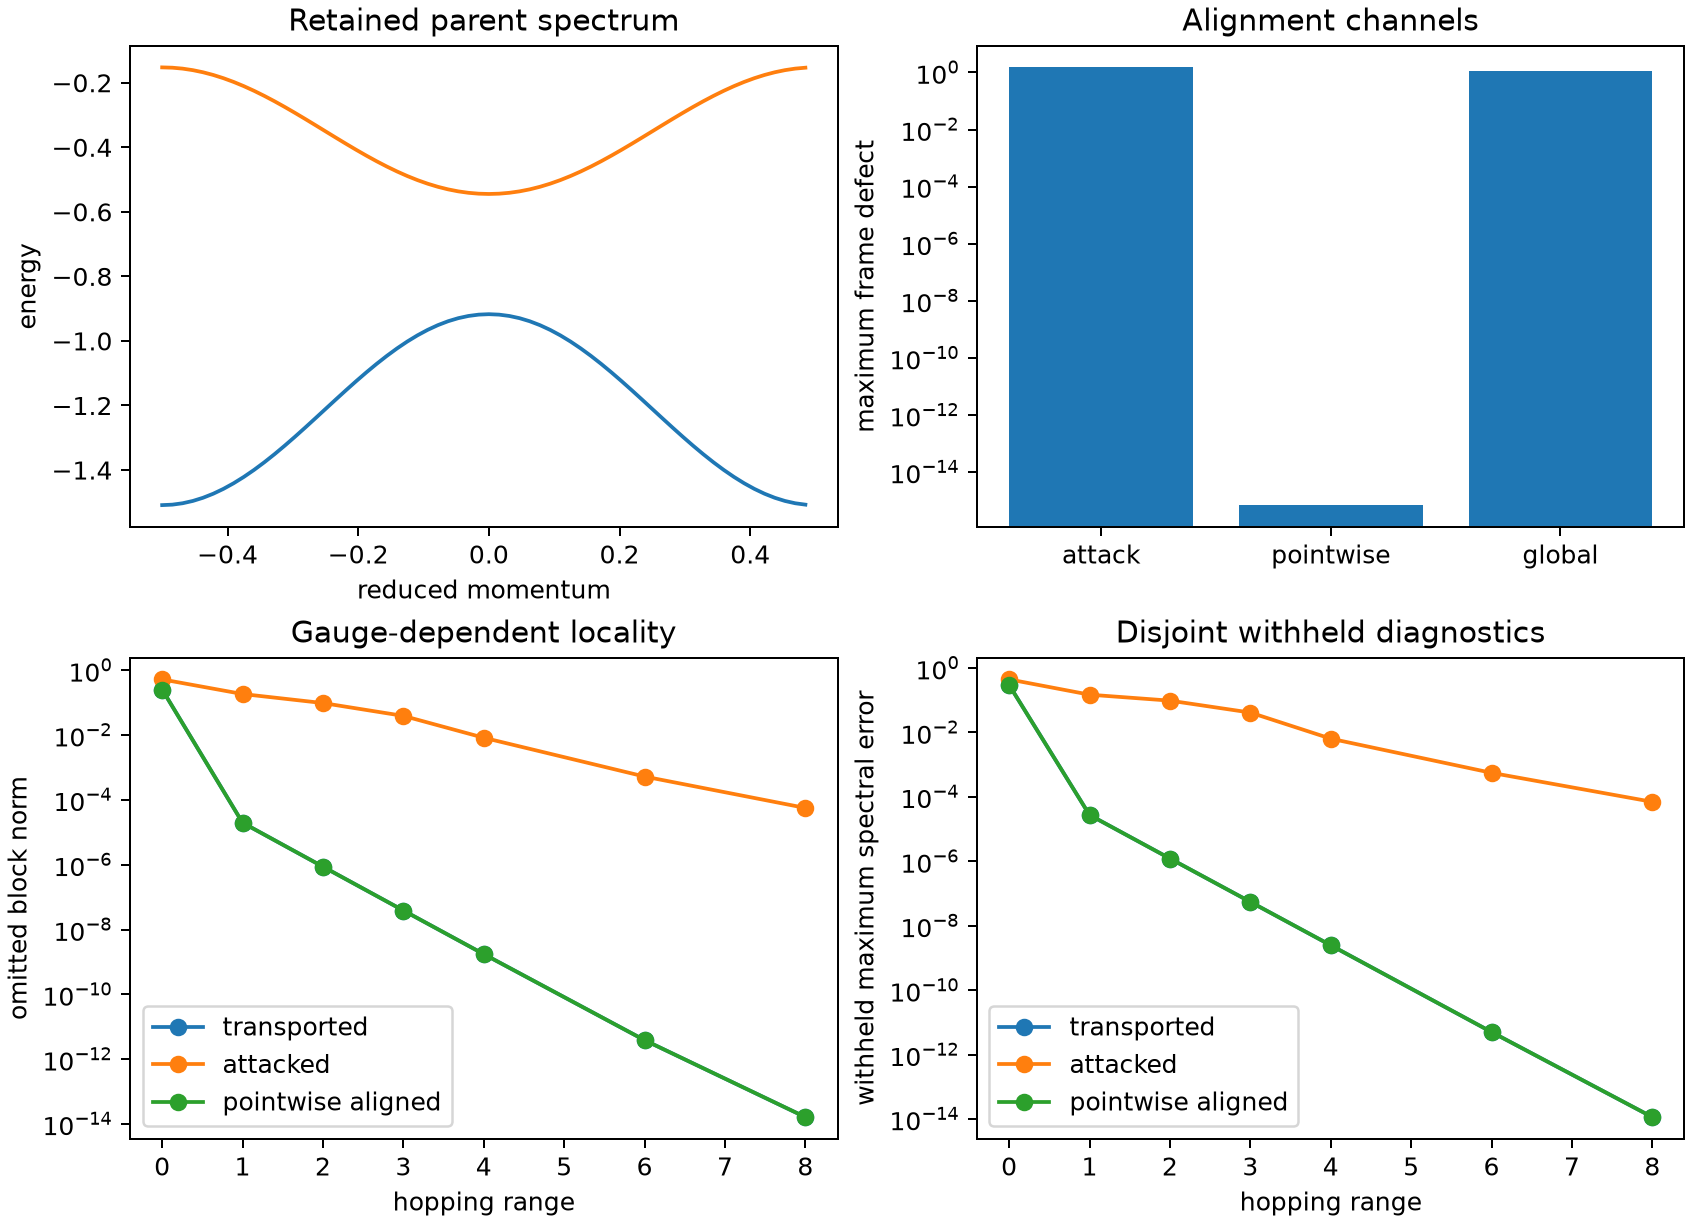
\includegraphics[width=0.97\linewidth]{../../../../../calculations/ICMSEP2026/conference/paper_1/multiband-alignment/multiband-alignment-summary.png}
 \caption{Frozen M2 retained spectrum, alignment channels, omitted block norms,
 and disjoint withheld maximum spectral errors. The exact pointwise channel is
 distinct from the one-global-unitary constrained family.}
 \label{fig:supp-m2-summary}
\end{figure}

\subsection{Gauge-resolved truncation and withheld checks}

Symmetric truncations retain representatives $|R|\leq R_{\max}$. Table
\ref{tab:supp-m2-ranges} reports selected values from the frozen range
sequence. The transported and pointwise-aligned frames recover the same local
behavior to floating-point error. In the attacked frame,
\[
 \widetilde H(k)=A(k)^\dagger H(k)A(k).
\]
Writing $H(k)=\sum_R e^{2\pi i kR}T_R$ and
$A(k)=\sum_m e^{2\pi i km}A_m$ gives the Fourier convolution
\[
 \widetilde T_Q=\sum_{m,n}A_m^\dagger T_{Q+m-n}A_n.
\]
A momentum-dependent unitary therefore mixes hopping coefficients across
ranges even though it preserves each fiber spectrum and retained projector; a
constant unitary has only its zero Fourier mode and merely conjugates each
block. Thus spectral and projector agreement do not protect finite-range
tight-binding locality or compressibility. The periodic attack redistributes
the same spectral information into a longer block-hopping tail. At range eight,
its omitted-block norm is $5.65\times10^{-5}$ and its withheld maximum spectral
error is $7.04\times10^{-5}$, compared with approximately
$1.6\times10^{-14}$ and $1.2\times10^{-14}$ for the transported channel.

\begin{table}[t]
\centering
\scriptsize
\caption{Selected M2 omitted-block norms and withheld maximum spectral errors.}
\label{tab:supp-m2-ranges}
\begin{tabular}{@{}rrrrrr@{}}
\toprule
$R_{\max}$ & $\|T\|_{\mathrm{omit}}$ & $\|\widetilde T\|_{\mathrm{omit}}$
& transported error & attacked error & aligned error\\
\midrule
0 & $2.54\!\times\!10^{-1}$ & $5.23\!\times\!10^{-1}$
  & $2.98\!\times\!10^{-1}$ & $4.45\!\times\!10^{-1}$ & $2.98\!\times\!10^{-1}$\\
1 & $1.98\!\times\!10^{-5}$ & $1.85\!\times\!10^{-1}$
  & $2.76\!\times\!10^{-5}$ & $1.49\!\times\!10^{-1}$ & $2.76\!\times\!10^{-5}$\\
4 & $1.75\!\times\!10^{-9}$ & $8.28\!\times\!10^{-3}$
  & $2.49\!\times\!10^{-9}$ & $6.43\!\times\!10^{-3}$ & $2.49\!\times\!10^{-9}$\\
8 & $1.63\!\times\!10^{-14}$ & $5.65\!\times\!10^{-5}$
  & $1.15\!\times\!10^{-14}$ & $7.04\!\times\!10^{-5}$ & $1.15\!\times\!10^{-14}$\\
\bottomrule
\end{tabular}
\end{table}

Withheld values evaluate only already fixed finite-range models. They do not
alter the parent, frame transport, attack, alignment family, hopping ranges,
thresholds, or figure-data selection.

\subsection{Independent verification and provenance}

The retained verifier independently rebuilds the parent polynomial,
eigenspaces, polar transport, periodic attack, pointwise and global
alignments, projected operators, Fourier blocks, Hermiticity defects,
truncations, omitted norms, and training/withheld spectral errors. Its maximum
dimensionless defect is $1.33\times10^{-15}$ and its maximum energy-channel
defect is $7.43\times10^{-15}$, both below the frozen $10^{-11}$ tolerance.

The input and protocol were hashed before the confirmatory calculation. The
package retains the protocol freeze, result, independent verification,
figure-data CSV, figure, report, software environment, source manifest, and
artifact checksums. The software record reports Python 3.14.6, NumPy 2.5.1,
SciPy 1.18.0, Matplotlib 3.11.1, and \texttt{ksdft2effmass 0.1.0.dev0}; the
dirty worktree is bound by \texttt{source.sha256}. No external calculator was
invoked.

\clearpage
\section*{Appendix S4. Wannier90 bridge calculation}
\label{supp:wannier90-bridge}
\renewcommand{\theequation}{S4.\arabic{equation}}
\setcounter{equation}{0}
\renewcommand{\thetable}{S4.\arabic{table}}
\setcounter{table}{0}
\renewcommand{\thefigure}{S4.\arabic{figure}}
\setcounter{figure}{0}

\subsection*{S4.1 Role and evidence boundary}

This appendix connects the controlled gauge-locality mechanism to retained
Wannier90 executions. It does not redefine M2. The balanced calculation is the
synthetic, non-DFT record
\path{research-monograph.periodic-2d.wannier90-balanced.v1} under
\path{calculations/research-monograph/periodic-2d/}. The parent is a finite
plane-wave representation of
\begin{equation}
 H=-\nabla^2+0.5\cos x+0.5\cos y+0.15\cos x\cos y
 \label{eq:supp-s4-parent}
\end{equation}
with a $15\times15\times1$ reciprocal mesh and a retained lowest-three-band
subspace. Wannier90 3.1.0 used centered $s$, $p_x$, and $p_y$ trial
projections; no disentanglement was used.

The external execution was historically authorized and retained. It is not
rerun by this manuscript. Repository-only verification consumes the compact
portable fixture and reconstructs the comparison independently of the
extractor. Passing establishes bounded consistency for this synthetic finite
interface, not first-principles, material, or general Wannier90 validation.

\subsection*{S4.2 Converged finite case and common-space alignment}

After a retained failed preprocessing attempt, the balanced auxiliary embedding
completed preprocessing and localization. Localization satisfied the frozen
$10^{-12}$ spread criterion at iteration 94. The direct projected frame and the
Wannier90 frame span the same retained subspace within a maximum projector
Frobenius defect of $2.65\times10^{-10}$.

Their raw represented Hamiltonians differ by $1.137E_G$ in maximum Frobenius
norm. Let $U_{\mathrm d}(\bm k)$ and $U_{\mathrm W}(\bm k)$ denote the direct
and Wannier90 frames. The pointwise unitary identification derived from those
frames reduces the represented-operator defect to
$3.57\times10^{-10}E_G$. By contrast, the frozen bounded family consisting of
independent integer orbital translations in $[-1,1]^2$ followed by one constant
orbital unitary leaves a per-orbital frame RMS defect of $1.188$ and an operator
defect of $1.490E_G$. Thus the observed relation is genuinely
$\bm k$-dependent within this comparison contract; it is not explained by a
single orbital rotation and bounded relabeling of orbital cells.

\subsection*{S4.3 Localization and hopping locality}

Native Wannier90 Berry-link spreads and common finite-supercell spreads use
different estimators and are not substituted for one another. The native total
active-plane spread is $0.7094a^2$. Under the common finite-supercell estimator,
the Wannier90 total is $6.1359a^2$ and the direct projected total is
$24.5163a^2$, giving a ratio of $0.2503$ for this finite case.

The same frame change also affects matrix-hopping tails. At squared-radius
shell 18, the omitted Frobenius $\ell^2$ norm is
$9.92\times10^{-3}E_G$ for the Wannier90 frame and
$1.38\times10^{-2}E_G$ for the direct projected frame. At shell 50 the values
are $2.72\times10^{-4}E_G$ and $5.90\times10^{-3}E_G$, respectively. These
commensurate diagnostics support the expected connection between localized
frames and shorter represented hopping tails for the frozen case. They do not
establish an optimality theorem.

The native \path{_hr.dat} blocks reconstruct the external mesh within
$3.06\times10^{-5}E_G$ in maximum Frobenius norm and
$2.23\times10^{-5}E_G$ spectrally. Those defects are retained as finite decimal
serialization effects, not relabeled as hopping truncation.

\begin{figure}[t]
 \centering
 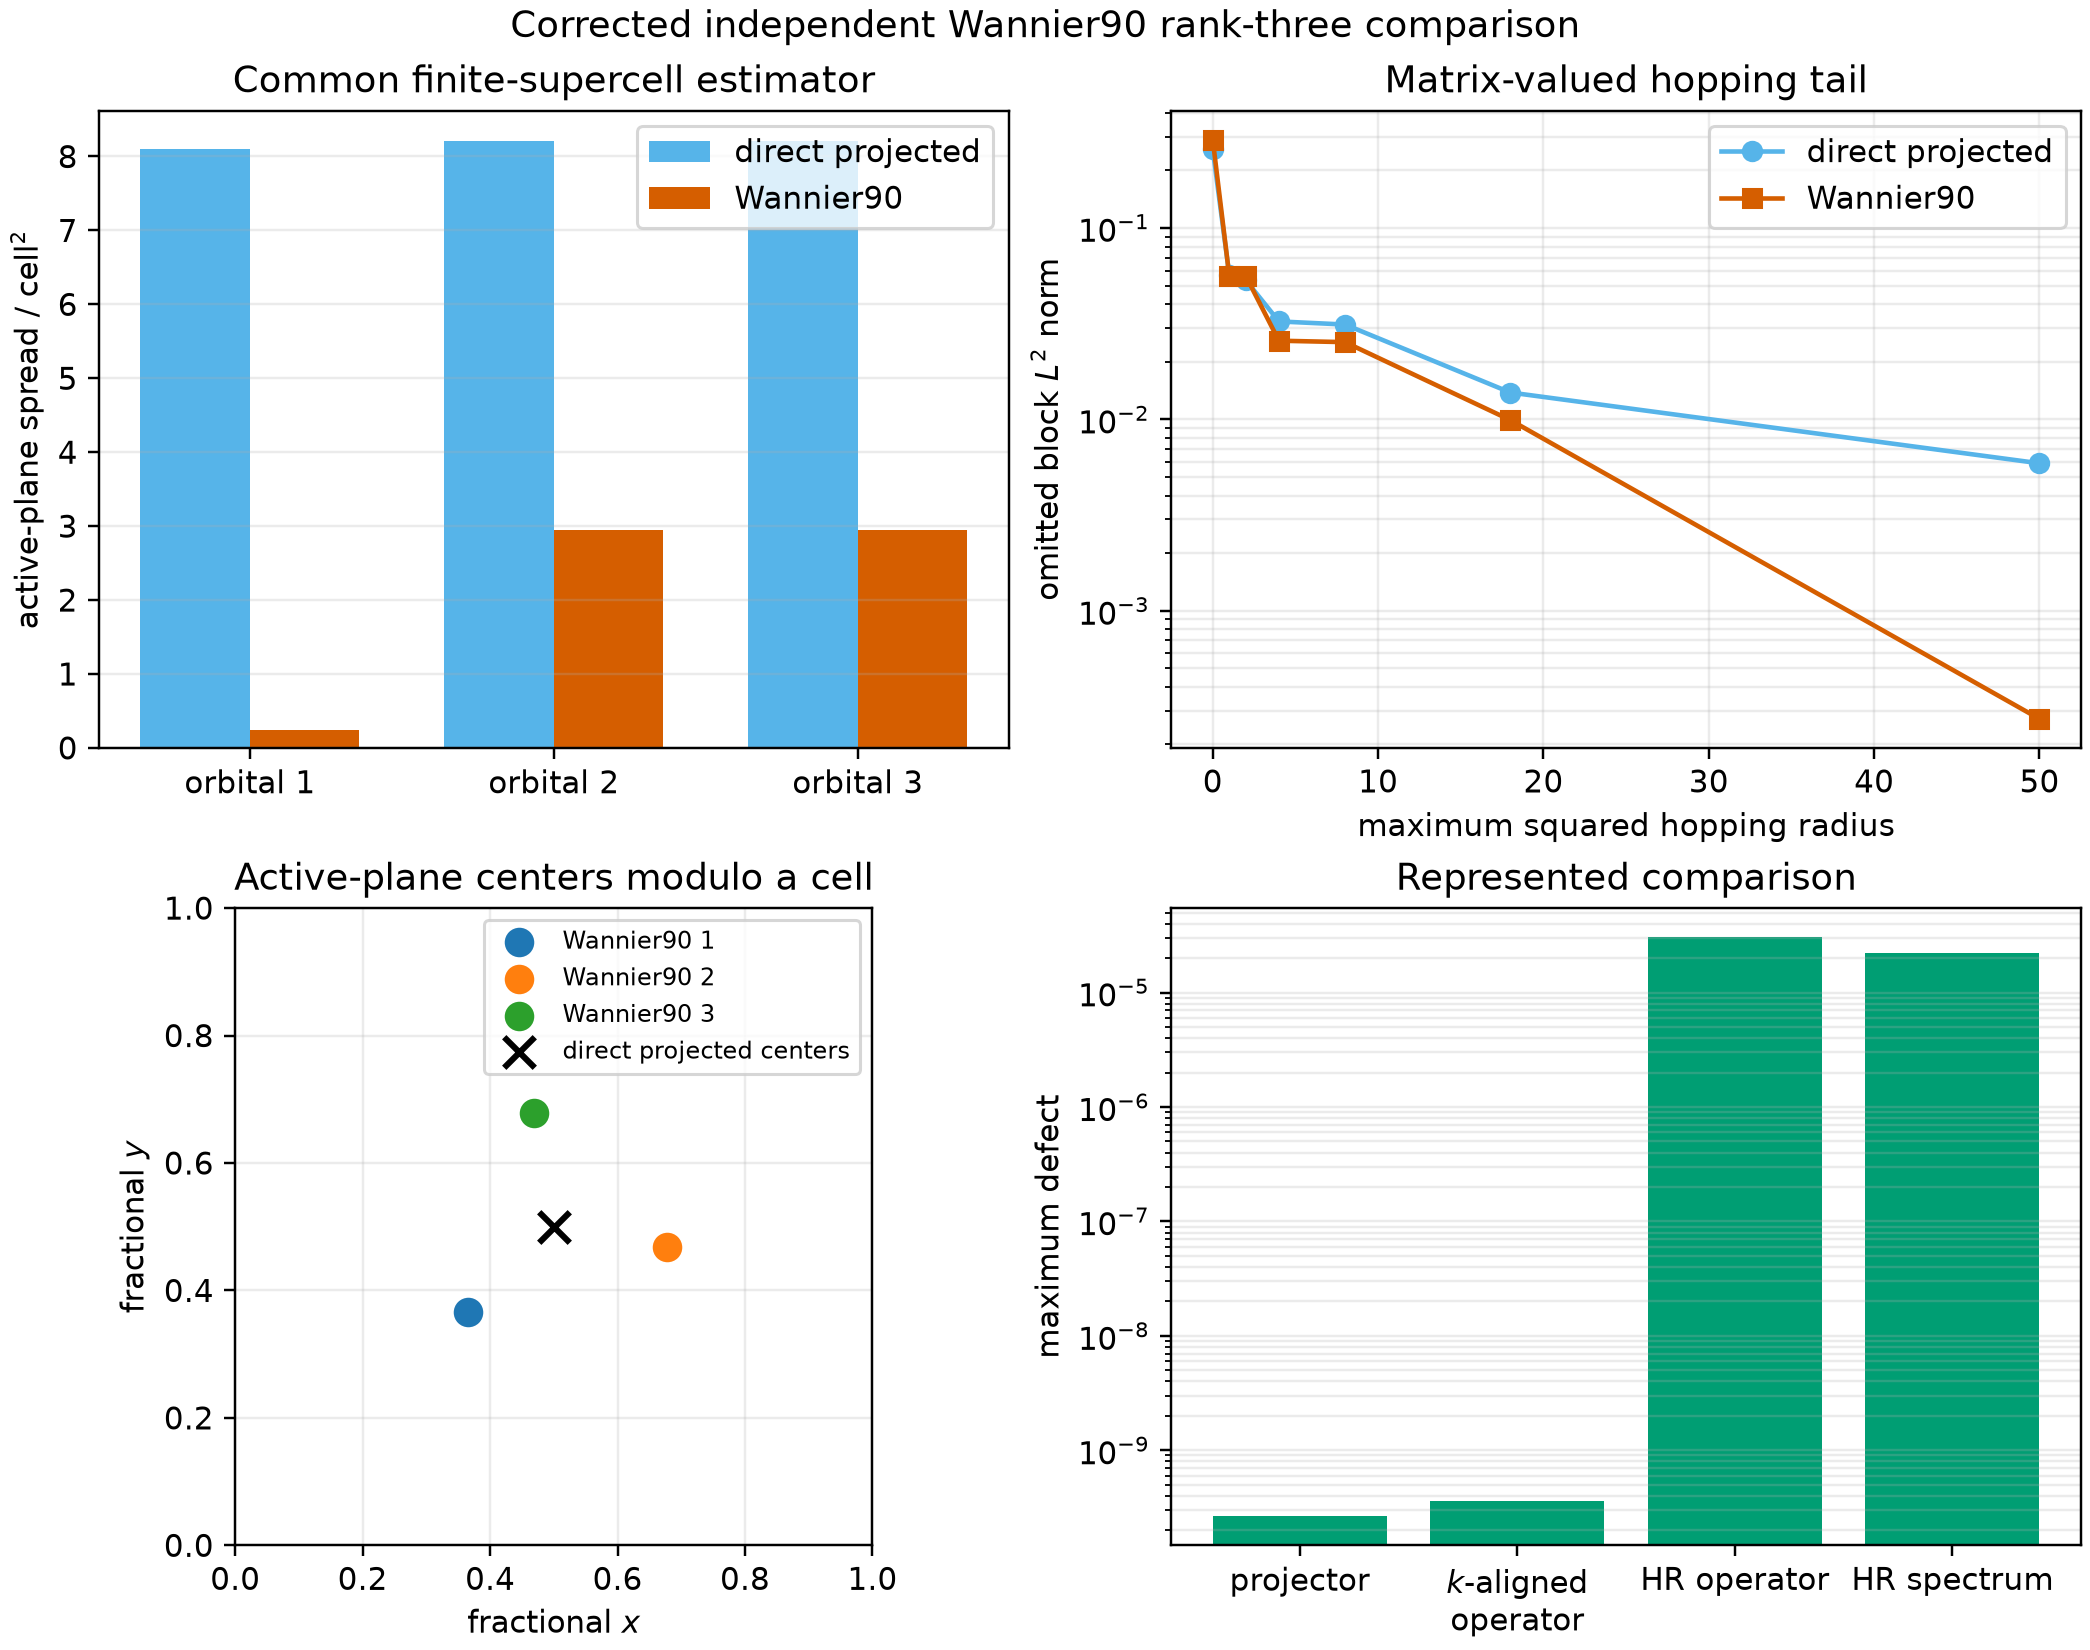
\includegraphics[width=0.97\linewidth]{../../../../../calculations/research-monograph/periodic-2d/wannier90-balanced-summary.png}
 \caption{Retained balanced Wannier90 comparison. Native and common-estimator
 spreads remain separate; aligned operator and shell-tail channels are evaluated
 on declared common representations.}
 \label{fig:supp-s4-wannier90-balanced}
\end{figure}

\subsection*{S4.4 Sensitivity study and interpretation limit}

A separately retained six-case study varies one of reciprocal mesh, plane-wave
cutoff, or inactive embedding length at a time. All finite cases converged, but
the outcomes are nonmonotone. Table~\ref{tab:supp-s4-sensitivity} records the
native spread and radius-50 tail needed for the interpretation boundary.

\begin{table}[t]
\centering
\small
\caption{Selected retained Wannier90 sensitivity observations.}
\label{tab:supp-s4-sensitivity}
\begin{tabular}{@{}lrr@{}}
\toprule
Case & Native spread ($a^2$) & Radius-50 tail ($E_G$)\\
\midrule
Reference $P3,N15,c15$ & $0.7094$ & $2.72\times10^{-4}$\\
Mesh $N=19$ & $1.7901$ & $4.52\times10^{-2}$\\
Cutoff $P=2$ & $1.7072$ & $3.30\times10^{-2}$\\
Cutoff $P=4$ & $1.7024$ & $3.38\times10^{-2}$\\
Embedding $c=12$ & $0.7093$ & $2.72\times10^{-4}$\\
Embedding $c=18$ & $1.7024$ & $3.38\times10^{-2}$\\
\bottomrule
\end{tabular}
\end{table}

The $c=12$ case returns close to the reference, whereas $c=18$ reaches a
different localization basin. The cutoff and mesh observations likewise do not
form a convergence sequence. Accordingly, the balanced calculation is a
positive finite-case bridge between M2's gauge mechanism and an actual
Wannier90-selected frame, while the sensitivity study blocks any claim of
mesh-, cutoff-, embedding-, or basin-independent localization. Neither record
supports a Si:P, Si:B, bulk-silicon, or other material-specific locality bound.

\subsection*{S4.5 Verification and provenance}

The portable balanced verifier independently reconstructs the finite parent,
direct polar frame, subspace and represented-operator defects, bounded
translation-plus-constant alignment search, native hopping reconstruction,
shell tails, convergence record, and common-grid densities and spreads. The
portable sensitivity verifier checks all six retained cases. Both pass against
the retained records. The directory-level \path{SHA256SUMS} manifest verifies
the reports, results, portable evidence, scripts, and figures. As in Appendix
S2, the digests establish byte consistency relative to the retained manifest;
they are not by themselves an external timestamp or a material-validation
argument.

\clearpage
\section{M3 constrained admissible sets}
\label{app:m3-constrained-admissible-sets}

\subsection{The question M3 asks}

M2 showed that two matrix representations can have the same band energies and
retained projector while having very different hopping coefficients. The
difference comes from a momentum-dependent rotation of the retained orbital
frame. A separate rotation at every momentum point recovers the original M2
matrices almost exactly, but one constant rotation over the whole Brillouin zone
generally cannot.

M3 asks a narrower question:
\begin{quote}
Can one reduced Hamiltonian satisfy both the spectral and
represented-operator requirements when the candidate family and allowed
orbital alignments are fixed in advance?
\end{quote}
This is a compatibility question under a declared contract. It is not a claim
that the underlying physical systems are different or that no more general
alignment could reconcile their matrices.

\subsection{A two-knob candidate model}

M3 starts from the transported M2 reference Hamiltonian $H(k)$. Let
$\overline E(k)=\operatorname{tr}H(k)/2$ be its mean band energy. A candidate is
\[
 H_{s,\lambda}(k)
 =\overline E(k)I+sE_GI
 +\lambda\left[H(k)-\overline E(k)I\right],
\]
where $E_G=1$ in the parent energy unit. The two parameters have simple roles:
\begin{itemize}
 \item $s$ shifts both bands together;
 \item $\lambda$ changes their splitting about the mean; and
 \item $(s,\lambda)=(0,1)$ is the original reference model.
\end{itemize}
The frozen search rectangle is
\[
 -0.25\leq s\leq0.25,
 \qquad
 0.4\leq\lambda\leq1.2.
\]
For matrix comparison, M3 allows only nine constant real rotations, with angles
from $-1.2$ to $1.2$ radians. It does not allow the momentum-dependent
pointwise alignment that recovers M2 exactly.

\subsection{Two accepted regions}

Each candidate receives two normalized RMS scores:
\begin{enumerate}
 \item \emph{spectral loss}, measuring disagreement between ordered band
 energies; and
 \item \emph{operator loss}, measuring matrix disagreement after the best
 allowed constant rotation.
\end{enumerate}
A threshold on each score produces a region in the $(s,\lambda)$ plane. The
spectral admissible set contains candidates passing the spectral threshold. The
operator admissible set is the union of the passing regions for the nine
rotation angles.

The decision rule is geometric. A retained point belonging to both regions
proves compatibility. Failure to find such a point proves nothing by itself. A
positive lower bound on the distance between the complete frozen regions
certifies separation.

Only the 64 training points define these regions and their quadratic
boundaries. The 257 staggered evaluation coordinates are disjoint from training
and are used only after the decision objects have been fixed.

\subsection{How the thresholds were chosen}

The thresholds are benchmark-design controls, not physical tolerances. They
were chosen from the known synthetic model and its preparatory analytic
training-loss geometry to produce two deliberately different decision regimes.

\begin{table}[ht]
\centering
\small
\caption{Design roles of the M3 thresholds and resolution.}
\begin{tabular}{@{}p{0.25\linewidth}p{0.67\linewidth}@{}}
\toprule
Control & Design role \\
\midrule
Spectral threshold $0.03$
 & Keeps spectral acceptance near the original splitting and places its
 minimum accepted splitting at approximately $0.9354687052$. \\
Compatible operator threshold $0.33$
 & Lies just above the original model's constrained operator loss
 $0.3286318914$, so $(0,1)$ is a common witness. \\
Separated operator threshold $0.31$
 & Shrinks operator acceptance until its maximum splitting is approximately
 $0.8360013041$. \\
Separation resolution $0.05$
 & Declares the minimum parameter-space gap that this benchmark will call
 resolved. \\
\bottomrule
\end{tabular}
\end{table}

Thus the separated design was required to satisfy
\[
 0.9354687052-0.8360013041
 =0.0994674010>0.05.
\]
The thresholds were frozen before the retained confirmatory execution, but
their selection was not blind. They were not inferred from withheld values,
experimental uncertainty, literature tolerances, or material acceptance
criteria. The calculation therefore demonstrates the decision procedure; it
does not calibrate universal thresholds.

An explicitly post-hoc analytic reanalysis varies only the operator threshold
while holding $\tau_S=0.03$. The operator set first becomes feasible at
approximately $0.307420$. Its distance from the spectral set exceeds the
declared $0.05$ resolution until $\tau_O=0.313791$, remains positive but below
resolution until the exact compatibility transition at $\tau_O=0.319264$, and
is compatible thereafter. The original point $(0,1)$ itself becomes
operator-admissible at $0.328632$. Thus the two designed thresholds lie
transparently on opposite sides of the transition rather than serving as
estimates of a physical tolerance. Its hardened verifier correlates the
consumed M3 result to the exact source-manifest entry and checks the zero-shift,
axis-alignment, symmetry, and positive-curvature premises used by this
reduction.

\begin{figure}[ht]
 \centering
 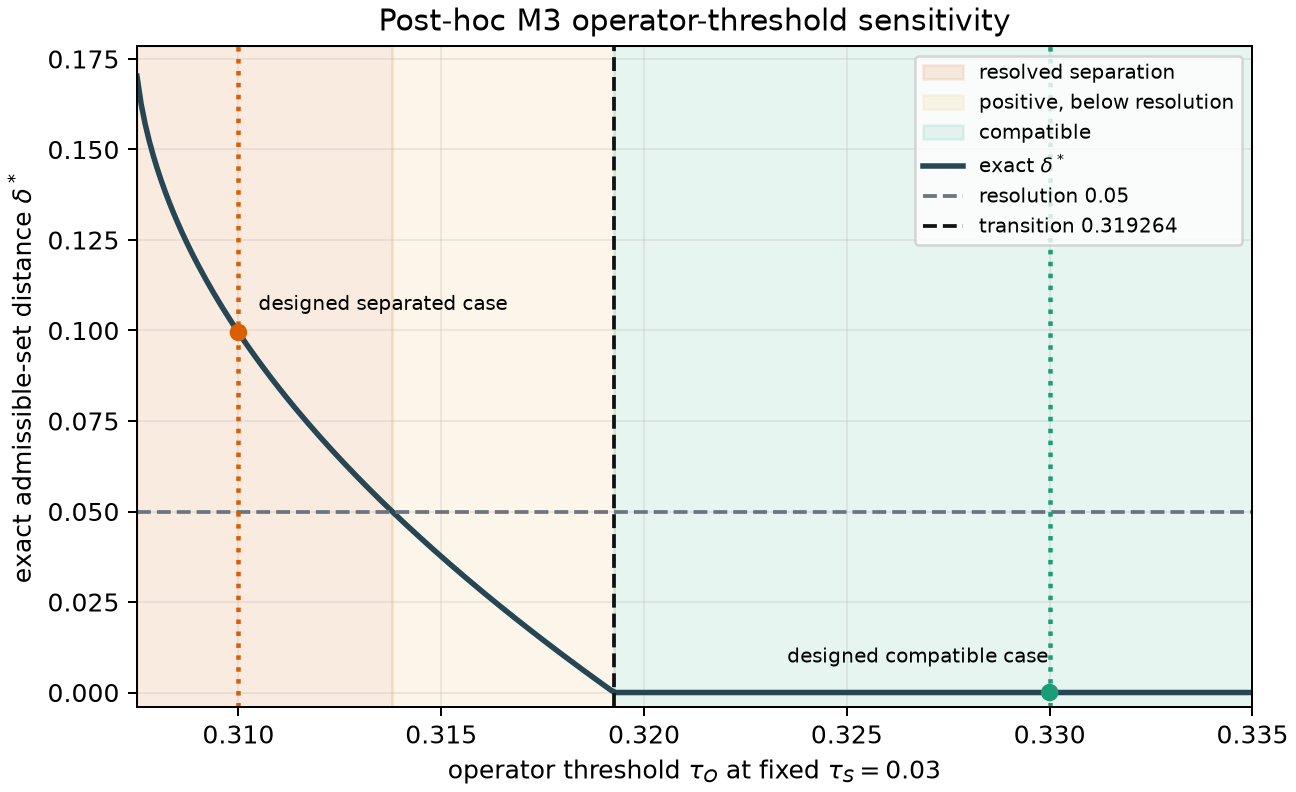
\includegraphics[width=0.96\linewidth]{../../../../../calculations/ICMSEP2026/conference/paper_1/constrained-admissible-sets-threshold-sensitivity/operator-threshold-sensitivity.png}
 \caption{Explicitly post-hoc M3 operator-threshold sensitivity at fixed
 $\tau_S=0.03$. The curve distinguishes resolved separation, positive distance
 below the declared resolution, and compatibility.}
 \label{fig:m3-threshold-sensitivity}
\end{figure}

\subsection{Compatible thresholds}

The first thresholds are
\[
 \tau_S=0.03,
 \qquad
 \tau_O=0.33.
\]
The original model $(0,1)$ passes both tests when the constant rotation angle is
$0.3$:
\begin{itemize}
 \item training spectral loss: $7.59\times10^{-16}$; and
 \item training operator loss: $0.3286318914$.
\end{itemize}
Because M3 retains this explicit common witness, the distance between the two
accepted regions is exactly zero. This is stronger than reporting that a
numerical search happened to find a small loss.

\subsection{Tightened operator threshold}

The second case keeps the spectral threshold at $0.03$ but tightens the operator
threshold to $0.31$. Within the frozen parameter rectangle and nine-angle
alignment family,
\begin{align*}
 \text{spectral acceptance}&:\quad \lambda\gtrsim0.9354687052,\\
 \text{operator acceptance}&:\quad \lambda\lesssim0.8360013041.
\end{align*}
The closest retained boundary points are therefore
\[
 p_S\approx(0,\,0.9354687052),
 \qquad
 p_O=(0,\,0.8360013041).
\]
Their Euclidean distance is
\[
 \lVert p_S-p_O\rVert_2=0.0994674010.
\]
The analytic quadratic certificate gives the same value as both a lower and a
constructive upper bound. Because it exceeds the prospectively frozen
resolution $0.05$, the retained disposition is \emph{certified separated}.

\begin{figure}[ht]
 \centering
 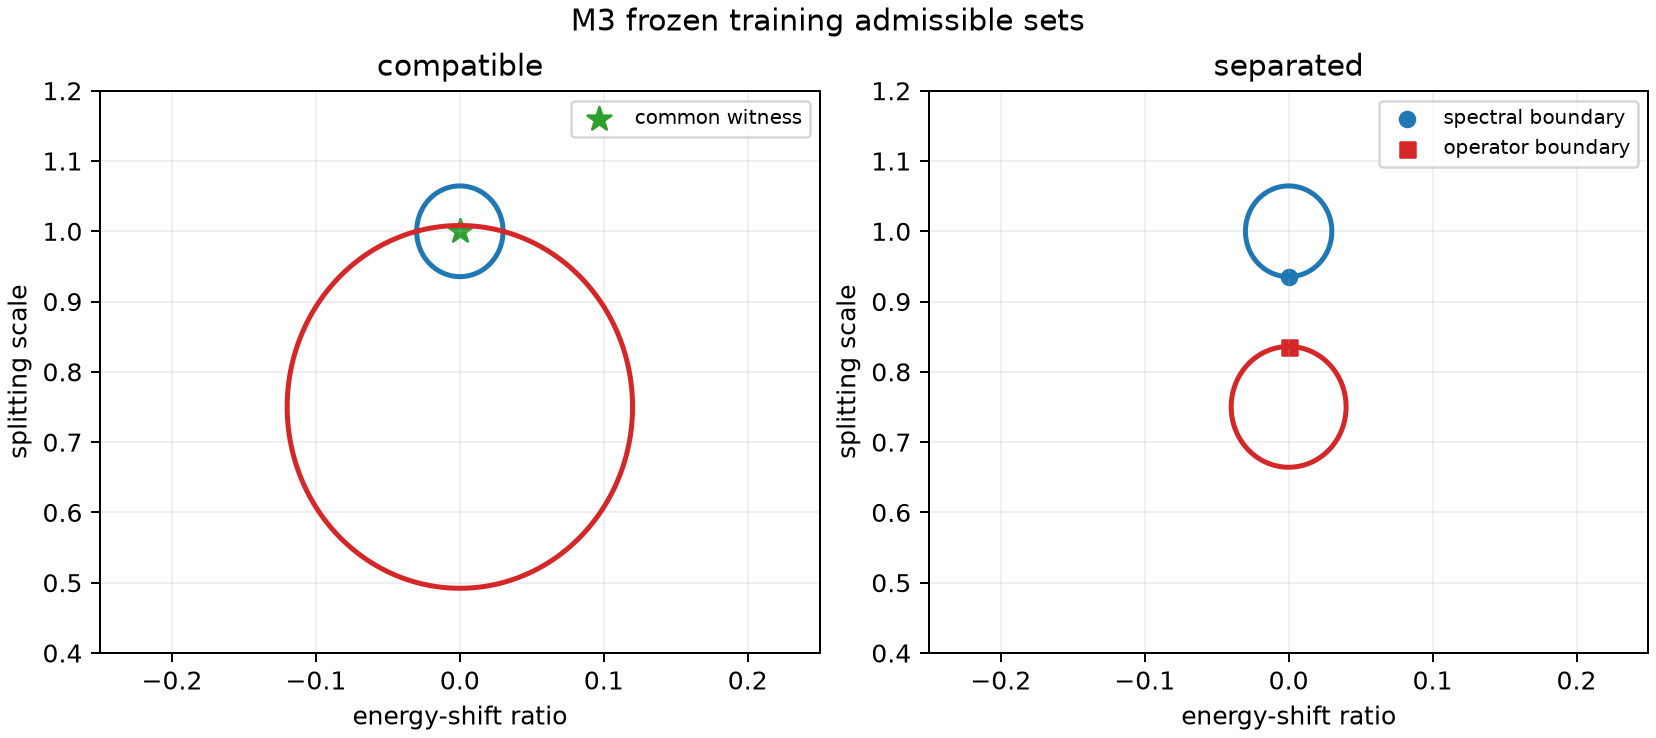
\includegraphics[width=0.96\linewidth]{../../../../../calculations/ICMSEP2026/conference/paper_1/constrained-admissible-sets/constrained-admissible-sets-summary.png}
 \caption{M3 constrained admissible sets. The compatible thresholds admit the
 original model as a common witness. Tightening the operator threshold leaves a
 certified gap between the spectral and operator regions.}
 \label{fig:m3-constrained-admissible-sets}
\end{figure}

\subsection{What the result does and does not mean}

M3 demonstrates that spectral and matrix requirements can select nonoverlapping
parts of the same reduced-model family when the alignment family and tolerances
are fixed. The result depends on the two-parameter model, nine constant
rotations, thresholds, Euclidean metric, finite meshes, and
quadratic-certificate assumptions.

It does not establish material validity, uncertainty quantification, silicon
transferability, or incompatibility under arbitrary momentum-dependent
alignments. In particular, M2 already shows that pointwise alignment can
recover the constructed frame attack almost exactly.

Before confirmatory evaluation, the editable TOML configuration, deterministic
input builder, derived input, M2 input digest, implementation sources, runner,
and standalone verifier were bound by \path{protocol-freeze.json}. Nine
retained amendments record post-freeze corrections and boundary hardening;
amendment 6 retracts an earlier incorrect diagnosis of a shared
training/evaluation coordinate, and amendment 9 records post-result role and
tolerance verification hardening without changing scientific controls or
numerical results.

The library verifier reports maximum dimensionless defect
$1.33\times10^{-15}$. The standalone verifier, which imports no producer
Actions, reports $4.66\times10^{-15}$, below the frozen $10^{-11}$ tolerance.
It nevertheless shares NumPy, SciPy, eigensolvers, floating-point behavior, and
scientific conventions with the producer. SHA-256 binds recorded bytes but does
not independently establish chronology.


\section*{Nomenclature}
\begin{table}[ht]
\centering
\begin{tabular}{@{}lll@{}}
\toprule
Symbol & Description & Unit \\
\midrule
$a$ & Lattice period & model length \\
$\mathfrak{A}_E,\mathfrak{A}_H$ & Spectral and operator admissible sets & -- \\
$\bm{C}$ & Admissible coordinate alignment & -- \\
$d_{\mathrm{red}}$ & Canonical reduced-parameter distance & -- \\
$E_G$ & Controlled-model reciprocal energy scale & model energy \\
$\bm{H}(\bm{k})$ & Represented Bloch Hamiltonian & energy \\
$\mathcal{L}_E,\mathcal{L}_H$ & Spectral and operator losses & dimensionless \\
$\mathcal{L}_{H,\mathrm{orb}}$ & Gauge-orbit operator loss & dimensionless \\
$\mathcal{L}_{H,\mathrm{frame}}$ & Frame-dependent excess loss & dimensionless \\
$\mathfrak{M}_j$ & Candidate reduced-model class & -- \\
$m$ & Controlled-model reference mass & model mass \\
$O_m$ & Declared scalar observable & observable dependent \\
$\mathcal{S}_H$ & Operator-comparison translation domain & -- \\
$\bm{\theta}$ & Canonical reduced-model parameters & mixed \\
$\tau_E,\tau_H$ & Admissibility thresholds & dimensionless \\
$\lambda_{xy}$ & Two-dimensional coupling amplitude & model energy \\
$\delta_j^\ast$ & Minimum admissible-set separation & -- \\
$\underline{\delta}_j,\overline{\delta}_j$ & Separation bounds & -- \\
\bottomrule
\end{tabular}
\end{table}

\section*{Acknowledgments}
% Add verified funding, computing-resource, institutional, and technical
% acknowledgments before submission.
To be completed before submission.

\section*{Data and code availability}
The controlled-model protocols, retained result records, verification code,
figures, and checksum manifests are maintained in the project repository under
\path{calculations/ICMSEP2026/conference/paper_1/isolated-band/},
\path{calculations/ICMSEP2026/conference/paper_1/multiband-alignment/},
\path{calculations/ICMSEP2026/conference/paper_1/constrained-admissible-sets/},
\path{calculations/research-monograph/periodic-2d/}, and
\path{calculations/ICMSEP2026/conference/paper_1/}. These working repository
records are not yet a public archival deposit or DOI.

\bibliographystyle{elsarticle-num}
\bibliography{references}

\end{document}
